% ============================================================================
% Project Overwatch — Linux Userspace EDR
% Academic Project Report — LaTeX Source
% ============================================================================

\documentclass[12pt, a4paper]{report}

% ── Packages ────────────────────────────────────────────────────────────────
\usepackage[utf8]{inputenc}
\usepackage[T1]{fontenc}
\usepackage{times}                         % Times New Roman
\usepackage[margin=1in]{geometry}
\usepackage{setspace}                      % Line spacing
\usepackage{graphicx}
\usepackage{tabularx}
\usepackage{booktabs}
\usepackage{longtable}
\usepackage{array}
\usepackage{float}
\usepackage{caption}
\usepackage{subcaption}
\usepackage{listings}                      % Code listings
\usepackage{xcolor}
\usepackage{hyperref}
\usepackage{titlesec}
\usepackage{fancyhdr}
\usepackage{enumitem}
\usepackage{amsmath}
\usepackage{tikz}
\usetikzlibrary{shapes.geometric, arrows.meta, positioning, fit, calc}

% ── Page Style ──────────────────────────────────────────────────────────────
\pagestyle{fancy}
\fancyhf{}
\fancyhead[L]{\small Project Overwatch: Linux Userspace EDR}
\fancyhead[R]{\small 2025--26}
\fancyfoot[C]{\thepage}
\renewcommand{\headrulewidth}{0.4pt}
\renewcommand{\footrulewidth}{0pt}

% ── Chapter / Section Formatting ────────────────────────────────────────────
\titleformat{\chapter}[display]
  {\normalfont\Large\bfseries\centering}
  {\MakeUppercase{\chaptertitlename}\ \thechapter}{12pt}{\LARGE\MakeUppercase}
\titlespacing*{\chapter}{0pt}{-20pt}{20pt}

% ── Code Listing Style ──────────────────────────────────────────────────────
\definecolor{codebg}{rgb}{0.96,0.96,0.96}
\definecolor{codegreen}{rgb}{0.0,0.5,0.0}
\definecolor{codegray}{rgb}{0.5,0.5,0.5}
\definecolor{codeblue}{rgb}{0.0,0.0,0.7}

\lstdefinestyle{cstyle}{
    backgroundcolor=\color{codebg},
    commentstyle=\color{codegreen}\itshape,
    keywordstyle=\color{codeblue}\bfseries,
    stringstyle=\color{red!70!black},
    basicstyle=\ttfamily\footnotesize,
    breakatwhitespace=false,
    breaklines=true,
    captionpos=b,
    keepspaces=true,
    numbers=left,
    numbersep=5pt,
    numberstyle=\tiny\color{codegray},
    showspaces=false,
    showstringspaces=false,
    showtabs=false,
    tabsize=4,
    frame=single,
    language=C
}
\lstset{style=cstyle}

% ── Hyperref Setup ──────────────────────────────────────────────────────────
\hypersetup{
    colorlinks=true,
    linkcolor=black,
    citecolor=blue!60!black,
    urlcolor=blue!70!black,
    bookmarks=true,
    pdfauthor={},
    pdftitle={Project Overwatch — Linux Userspace EDR},
}

% ── Line Spacing ────────────────────────────────────────────────────────────
\onehalfspacing

% ============================================================================
\begin{document}

% ── TITLE PAGE ──────────────────────────────────────────────────────────────
\begin{titlepage}
    \centering
    \vspace*{1cm}

    {\Large\bfseries PROJECT OVERWATCH}\\[0.4cm]
    {\large\bfseries Linux Userspace Endpoint Detection and Response System}\\[0.3cm]
    {\large\bfseries Using ptrace-Based System Call Interception}

    \vspace{1.5cm}

    {\normalsize A Project Report Submitted in Partial Fulfillment of the\\
    Requirements for the Degree of}\\[0.5cm]
    {\large\bfseries Bachelor of Engineering}\\[0.3cm]
    {\normalsize in}\\[0.3cm]
    {\large\bfseries Information Science and Engineering}

    \vspace{1.5cm}

    {\normalsize\itshape Submitted by}\\[0.4cm]
    \begin{tabular}{c}
        \textbf{Student Name} \quad USN \\
    \end{tabular}

    \vspace{1.5cm}

    {\normalsize Under the Guidance of}\\[0.3cm]
    {\normalsize\bfseries Guide Name}\\
    {\normalsize Department of Information Science and Engineering}

    \vfill

    {\normalsize Department of Information Science and Engineering}\\[0.2cm]
    {\normalsize\bfseries RV College of Engineering\textsuperscript{\textregistered}}\\
    {\small Mysore Road, RV Vidyaniketan Post, Bengaluru -- 560059, Karnataka, India}\\
    {\small Affiliated to Visvesvaraya Technological University, Belagavi}\\[0.5cm]
    {\normalsize\bfseries 2025--26}
\end{titlepage}

% ── ABSTRACT ────────────────────────────────────────────────────────────────
\chapter*{Abstract}
\addcontentsline{toc}{chapter}{Abstract}

Endpoint Detection and Response (EDR) systems form a critical layer in modern cybersecurity infrastructure, providing real-time monitoring, threat detection, and automated response capabilities at the host level. However, most production EDR solutions operate as proprietary, kernel-level agents whose internal mechanisms remain opaque to students and security researchers. This project presents \textbf{Project Overwatch}, a fully transparent, userspace EDR prototype for Linux x86\_64 that leverages the \texttt{ptrace} debugging API to intercept, decode, inspect, and enforce security policies on system calls made by traced processes---all without requiring kernel modifications, loadable kernel modules, or elevated eBPF privileges.

Project Overwatch implements a four-phase pipeline: (1)~\textbf{Process Instrumentation} spawns or attaches to a target process using \texttt{fork()}, \texttt{PTRACE\_TRACEME}, and \texttt{execvp()}, establishing a parent--child tracing relationship mediated by the kernel's \texttt{waitpid}/\texttt{ptrace} protocol; (2)~\textbf{Syscall Decoding} reads the frozen process's CPU registers via \texttt{PTRACE\_GETREGS} and maps the x86\_64 System~V ABI register layout (RAX, RDI, RSI, RDX, R10, R8, R9) to human-readable syscall names and categories (FILE, NETWORK, PROCESS, SYSTEM); (3)~\textbf{Memory Inspection} crosses the virtual memory isolation barrier using \texttt{PTRACE\_PEEKDATA} to reconstruct file paths, socket addresses, and \texttt{argv} arrays from the traced process's address space; and (4)~\textbf{Heuristic Enforcement} evaluates each intercepted syscall against a rule engine of twelve detection rules covering credential theft, privilege escalation, persistence mechanisms, defense evasion, and suspicious network connections, producing graduated responses from logging through alerting to process termination.

The system was validated against three purpose-built test programs simulating benign file access, network socket operations, and adversarial behaviors (shadow file reading, SSH key exfiltration, \texttt{/proc/self/mem} access, cron persistence). Results demonstrate successful interception of all syscalls, accurate cross-process string reconstruction, correct rule triggering across all threat categories, and reliable process termination in enforcement mode. The report discusses architectural trade-offs, known limitations (single-process tracing, stub blocking, partial network coverage), and concrete extension paths toward descendant-aware, multi-threaded, production-grade EDR capabilities.

\vspace{0.5cm}
\noindent\textbf{Keywords:} Endpoint Detection and Response, ptrace, system call tracing, Linux security, userspace monitoring, heuristic enforcement, x86\_64 ABI, process instrumentation.

% ── TABLE OF CONTENTS ───────────────────────────────────────────────────────
\tableofcontents
\listoffigures
\listoftables

% ============================================================================
%                           CHAPTER 1: INTRODUCTION
% ============================================================================
\chapter{Introduction}

\section{Project Overview}

Project Overwatch is a userspace Endpoint Detection and Response (EDR) prototype for Linux x86\_64 systems. It demonstrates how security monitoring tools can intercept and analyze process behavior at the system call level using the \texttt{ptrace} debugging API, without requiring kernel modifications, loadable kernel modules (LKMs), or eBPF programs.

The system operates on a fundamental principle of operating systems: every meaningful action a user-space program takes---opening a file, creating a network connection, spawning a child process, or modifying permissions---must pass through the kernel via a \emph{system call}. By interposing on this narrow interface between user space and kernel space, Overwatch gains comprehensive visibility into a monitored process's behavior.

The project is implemented in approximately 2{,}100 lines of C11 code, organized into six source modules and one header file. It compiles with GCC under strict warning flags (\texttt{-Wall -Wextra -Werror}) and targets the x86\_64 Linux ABI exclusively.

\section{Purpose and Scope}

The purpose of Project Overwatch is threefold:

\begin{enumerate}[label=\arabic*.]
    \item \textbf{Educational Transparency.} To provide a clear, well-documented implementation of a ptrace-based syscall monitoring pipeline that students and security researchers can study, modify, and extend. Unlike production EDR agents (CrowdStrike Falcon, Microsoft Defender for Endpoint, Carbon Black), whose source code is proprietary, Overwatch exposes every decision point---from register extraction to rule evaluation to kill logic---in readable C with extensive comments.

    \item \textbf{Practical Demonstration.} To show that meaningful security monitoring is achievable in user space, using only standard POSIX and Linux APIs (\texttt{ptrace}, \texttt{waitpid}, \texttt{fork}, \texttt{execvp}, \texttt{kill}). This challenges the common assumption that all security tooling must live in kernel space.

    \item \textbf{Foundation for Extension.} To serve as a base platform for exploring advanced topics: multi-process tracing, syscall blocking via register rewriting, eBPF/seccomp pre-filtering, JSON-configurable rule engines, and network-layer deep packet inspection.
\end{enumerate}

\noindent The scope of the current implementation covers:
\begin{itemize}
    \item Single-process, single-thread syscall tracing from process birth to exit.
    \item Interception at the immediate \texttt{execve} boundary (the first program the traced process runs).
    \item Path-based and port-based heuristic rules for file, process, and network behaviors.
    \item Two operational modes: \emph{passive} (log and alert only) and \emph{enforce} (alert and terminate).
    \item Three sample test programs for validation.
\end{itemize}

\section{Key Features}

\begin{table}[H]
\centering
\caption{Key features of Project Overwatch}
\label{tab:features}
\begin{tabularx}{\textwidth}{l X}
\toprule
\textbf{Feature} & \textbf{Description} \\
\midrule
Syscall Interception & Traces every system call via \texttt{PTRACE\_SYSCALL} with double-stop (entry/exit) tracking \\
Register Decoding & Reads x86\_64 registers (RAX, RDI, RSI, RDX, R10, R8, R9, RIP) via \texttt{PTRACE\_GETREGS} \\
Cross-Process Memory Read & Reconstructs strings and structures from the tracee's virtual address space using \texttt{PTRACE\_PEEKDATA} \\
Syscall Categorization & Classifies each syscall into FILE, NETWORK, PROCESS, or SYSTEM with color-coded terminal output \\
Heuristic Rule Engine & 12 built-in detection rules with glob pattern matching (\texttt{fnmatch}) and five-level threat classification \\
Graduated Response & Actions range from ALLOW $\to$ LOG $\to$ ALERT $\to$ BLOCK $\to$ KILL \\
Enforcement Mode & Automatically terminates processes triggering HIGH/CRITICAL rules when \texttt{-e} flag is set \\
Session Statistics & Tracks and reports total syscalls, file accesses, network connections, executions, alerts, blocks, and kills \\
Signal Handling & Graceful shutdown on SIGINT/SIGTERM with clean \texttt{PTRACE\_DETACH} \\
\bottomrule
\end{tabularx}
\end{table}


% ============================================================================
%                        CHAPTER 2: PROBLEM DEFINITION
% ============================================================================
\chapter{Problem Definition}

\section{Problem Statement}

Modern computing environments face an escalating threat landscape characterized by sophisticated malware, advanced persistent threats (APTs), fileless attacks, and living-off-the-land techniques that exploit legitimate system utilities for malicious purposes. Endpoint Detection and Response (EDR) systems have emerged as a critical defensive layer, providing real-time visibility into host-level process behavior, automated threat detection, and rapid incident response capabilities.

However, understanding \emph{how} EDR systems work at a technical level remains a significant challenge for students, security researchers, and aspiring threat analysts. The core problem can be stated as:

\begin{quote}
\itshape
How can the fundamental mechanisms of endpoint detection and response---system call interception, argument decoding, cross-process memory inspection, and heuristic enforcement---be implemented transparently in Linux user space using only standard APIs, such that the resulting system serves as both a functional security monitor and an educational platform for understanding OS-level threat detection?
\end{quote}

\noindent This problem encompasses several technical sub-problems:

\begin{enumerate}[label=(\alph*)]
    \item \textbf{Process Instrumentation:} How to gain control over a target process's execution at every system call boundary without modifying the kernel or the target program's binary.
    \item \textbf{Semantic Decoding:} How to translate raw CPU register values at a syscall trap into meaningful, human-readable information (syscall name, file path, network address, process arguments).
    \item \textbf{Memory Barrier Crossing:} How to read data structures (strings, \texttt{sockaddr}, \texttt{argv} arrays) from a foreign process's virtual address space, given that virtual memory isolation prevents direct pointer dereferencing.
    \item \textbf{Behavioral Heuristics:} How to define and evaluate detection rules that identify suspicious behavior (credential access, persistence, defense evasion, lateral movement) based solely on syscall-level telemetry.
    \item \textbf{Response Enforcement:} How to take graduated defensive actions---from passive logging through active process termination---within the constraints of the ptrace API.
\end{enumerate}

\section{Problem Relevance}

\subsection{Educational Context}

Traditional computer science education addresses operating system concepts through theoretical discussion and study of production kernels, leaving students with limited practical understanding of host-level security monitoring. The challenge is profound: while undergraduate curricula thoroughly cover data structures, algorithms, and systems concepts in isolation, few educational initiatives integrate these concepts into a coherent, working security tool where students can observe how architectural decisions manifest as measurable system behavior.

Contemporary security education faces three interrelated gaps:

\begin{enumerate}[label=\arabic*.]
    \item \textbf{Opacity of Production Tools.} Commercial EDR agents (CrowdStrike, SentinelOne, Carbon Black) are closed-source, kernel-level systems whose detection logic, interception mechanisms, and response pipelines are invisible to learners.

    \item \textbf{Complexity Barrier.} Open-source security tools like \texttt{strace}, \texttt{auditd}, or Falco, while valuable, are either too narrow in scope (tracing only) or too complex in implementation (kernel modules, eBPF programs) for educational use.

    \item \textbf{Theory--Practice Disconnect.} Students learn about system calls, virtual memory, process control, and signals in separate courses but rarely see these concepts composed into a single, purposeful system.
\end{enumerate}

\noindent Project Overwatch addresses all three gaps by providing a readable, self-contained implementation that a student with basic C and Linux knowledge can compile, run, modify, and extend within a single lab session.

\subsection{Industrial Relevance}

From an industry perspective, the project addresses several practical concerns:

\begin{itemize}
    \item \textbf{SOC Analyst Training:} Security Operations Center analysts benefit from understanding the syscall-level telemetry that EDR tools generate. Overwatch produces the same categories of data (file access logs, network connection events, process execution chains, alert streams) that analysts encounter in production SIEM dashboards.

    \item \textbf{Threat Hunting:} The detection rules in Overwatch mirror real-world MITRE ATT\&CK techniques---T1003 (Credential Dumping via \texttt{/etc/shadow}), T1053 (Scheduled Task/Cron persistence), T1059 (Command-Line Interface via netcat), T1055 (Process Injection via \texttt{/proc/*/mem})---giving practitioners hands-on experience with behavioral detection logic.

    \item \textbf{Red Team / Blue Team Exercises:} The enforce vs.\ passive modes enable realistic attack--defense scenarios where one team develops evasion techniques (e.g., using \texttt{openat} instead of \texttt{open}, indirect syscalls, ptrace detection) while the other team extends the rule engine.

    \item \textbf{Prototype Development:} Security startups and research labs can use the Overwatch architecture as a rapid prototyping framework for novel detection algorithms before investing in kernel-level or eBPF implementations.
\end{itemize}


% ============================================================================
%                     CHAPTER 3: BACKGROUND INFORMATION
% ============================================================================
\chapter{Background Information}

\section{Historical Context}

\subsection{Evolution of Endpoint Security (1990s--2010s)}

Endpoint security evolved through distinct generations. First-generation antivirus (1990s) relied on static signature matching---comparing file byte sequences against databases of known malware hashes. Second-generation tools (2000s) added heuristic analysis and sandboxing, executing suspicious files in isolated environments to observe behavior. Third-generation Endpoint Protection Platforms (EPPs, 2010s) introduced machine learning classifiers and cloud-based reputation systems.

The critical inflection point came with the recognition that signature-based detection fails against zero-day exploits, polymorphic malware, and fileless attacks that never touch disk. This realization drove the creation of \emph{behavioral} detection---monitoring what programs \emph{do} rather than what they \emph{are}---which is the foundational principle of modern EDR.

\subsection{Modern EDR Systems (2013--Present)}

The term ``Endpoint Detection and Response'' was coined by Gartner analyst Anton Chuvakin in 2013. Modern EDR systems (CrowdStrike Falcon, Microsoft Defender for Endpoint, SentinelOne, Carbon Black) share a common architecture:

\begin{enumerate}[label=\arabic*.]
    \item \textbf{Sensor:} A kernel-level agent that hooks into syscall dispatch, file I/O, network stack, and process creation paths.
    \item \textbf{Telemetry Pipeline:} Streams of structured events (process creation, file modification, network connection, registry change) forwarded to a central analytics engine.
    \item \textbf{Detection Engine:} A combination of rule-based matching, statistical anomaly detection, and machine learning classifiers that evaluate event streams against known attack patterns.
    \item \textbf{Response Actions:} Automated or analyst-initiated containment actions: process kill, file quarantine, network isolation, or remediation scripts.
\end{enumerate}

\noindent Project Overwatch re-creates this four-stage pipeline entirely in user space using \texttt{ptrace}, demonstrating the same architectural principles at a comprehensible scale.

\section{Linux System Call Architecture}

\subsection{The System Call Interface}

A \emph{system call} (syscall) is the programmatic interface through which user-space programs request services from the operating system kernel. On Linux x86\_64, the \texttt{syscall} instruction triggers a mode switch from Ring~3 (user mode) to Ring~0 (kernel mode), transferring control to the kernel's syscall dispatch table.

The x86\_64 System~V ABI defines the following register convention for syscalls:

\begin{table}[H]
\centering
\caption{x86\_64 System Call Register Convention}
\label{tab:registers}
\begin{tabular}{lll}
\toprule
\textbf{Register} & \textbf{Purpose} & \textbf{Example (\texttt{open} syscall)} \\
\midrule
RAX & Syscall number (entry) / Return value (exit) & 2 (\texttt{SYS\_open}) \\
RDI & Argument 1 & Pointer to filename string \\
RSI & Argument 2 & Flags (\texttt{O\_RDONLY}) \\
RDX & Argument 3 & Mode (permissions) \\
R10 & Argument 4 & --- \\
R8  & Argument 5 & --- \\
R9  & Argument 6 & --- \\
RIP & Instruction pointer & Address of \texttt{syscall} instruction \\
\bottomrule
\end{tabular}
\end{table}

\noindent Linux x86\_64 defines over 330 system calls (as of kernel 6.x), each identified by a unique number. Project Overwatch's decoder module maps approximately 150 of the most common syscall numbers to human-readable names and descriptions.

\subsection{x86\_64 Privilege Levels}

The x86\_64 architecture defines four privilege levels (rings), though Linux uses only two:

\begin{itemize}
    \item \textbf{Ring 0 (Kernel Mode):} Full hardware access. The kernel, device drivers, and kernel modules run here.
    \item \textbf{Ring 3 (User Mode):} Restricted access. All user applications, including Project Overwatch, run here.
\end{itemize}

\noindent The \texttt{syscall} instruction is the controlled gate between these rings. This is precisely the choke point that Overwatch monitors: by trapping every transition from Ring~3 to Ring~0, we observe every kernel service request the target process makes.

\section{The ptrace Debugging API}

\subsection{ptrace Overview}

\texttt{ptrace} (``process trace'') is a Linux system call that allows one process (the \emph{tracer}) to observe and control the execution of another process (the \emph{tracee}). Originally designed for debuggers like GDB, \texttt{ptrace} provides the following capabilities exploited by Overwatch:

\begin{table}[H]
\centering
\caption{ptrace Operations Used by Project Overwatch}
\label{tab:ptrace}
\begin{tabularx}{\textwidth}{l X}
\toprule
\textbf{Operation} & \textbf{Purpose in Overwatch} \\
\midrule
\texttt{PTRACE\_TRACEME} & Called by the child process to volunteer for tracing by its parent \\
\texttt{PTRACE\_SYSCALL} & Resumes the tracee, stopping it at the next syscall entry or exit \\
\texttt{PTRACE\_GETREGS} & Reads the complete CPU register state (all 27 general-purpose registers) from the stopped tracee \\
\texttt{PTRACE\_PEEKDATA} & Reads one word (8 bytes) from the tracee's virtual address space \\
\texttt{PTRACE\_SETOPTIONS} & Configures tracing options (\texttt{O\_TRACESYSGOOD}, \texttt{O\_TRACEEXEC}) \\
\texttt{PTRACE\_KILL} & Terminates the tracee immediately \\
\texttt{PTRACE\_ATTACH} & Attaches to an already-running process \\
\texttt{PTRACE\_DETACH} & Releases the tracee, allowing normal execution \\
\bottomrule
\end{tabularx}
\end{table}

\subsection{The Tracing Lifecycle}

The ptrace tracing lifecycle follows a well-defined protocol:

\begin{enumerate}[label=\arabic*.]
    \item The parent process calls \texttt{fork()} to create a child.
    \item The child calls \texttt{ptrace(PTRACE\_TRACEME)} to opt into tracing.
    \item The child calls \texttt{raise(SIGSTOP)} to synchronize with the parent.
    \item The child calls \texttt{execvp()} to replace its memory image with the target program.
    \item The parent calls \texttt{waitpid()} to catch the child's stop.
    \item The parent sets options via \texttt{PTRACE\_SETOPTIONS}.
    \item The parent enters the interception loop: \texttt{PTRACE\_SYSCALL} $\to$ \texttt{waitpid()} $\to$ inspect $\to$ decide $\to$ resume.
\end{enumerate}

\subsection{The Double-Stop Phenomenon}

A critical concept in ptrace-based syscall tracing is the \emph{double-stop phenomenon}. When \texttt{PTRACE\_SYSCALL} is used, the kernel stops the tracee \emph{twice} for each system call:

\begin{itemize}
    \item \textbf{Entry Stop:} The tracee is paused \emph{before} the kernel processes the syscall. Registers contain the syscall number and arguments. This is the ideal point for inspection and policy decisions.
    \item \textbf{Exit Stop:} The tracee is paused \emph{after} the kernel completes the syscall. RAX now contains the return value (e.g., a file descriptor or an error code).
\end{itemize}

\noindent Project Overwatch tracks entry vs.\ exit using a boolean toggle (\texttt{ctx->in\_syscall}), performing detection logic only on entry stops and logging return values on exit stops.

\section{Virtual Memory and Cross-Process Inspection}

Each Linux process has its own virtual address space, enforced by the Memory Management Unit (MMU). Address \texttt{0x7ffd12345678} in the tracee maps to a completely different physical page than the same virtual address in the tracer. This \emph{virtual memory isolation} is a fundamental security property of modern operating systems.

When Overwatch intercepts a syscall like \texttt{open(0x7ffd12345678, O\_RDONLY)}, the first argument is a \emph{pointer to a string in the tracee's address space}. The tracer cannot dereference this pointer directly---doing so would either segfault or read garbage from its own address space.

The solution is \texttt{PTRACE\_PEEKDATA}, which asks the kernel to read one word (8~bytes on x86\_64) from the tracee's memory and return it to the tracer. Overwatch's memory module reads words iteratively, scanning for null terminators to reconstruct complete C strings from across the process boundary.

\section{Heuristic Threat Detection}

Heuristic detection identifies threats by analyzing \emph{behavior patterns} rather than matching known signatures. The approach is grounded in the observation that malicious programs, regardless of their binary composition, must eventually interact with the operating system through system calls to achieve their objectives.

Common behavioral indicators that Overwatch monitors include:

\begin{itemize}
    \item \textbf{Credential Access:} Reading \texttt{/etc/shadow} (password hashes), \texttt{/etc/passwd} (user accounts), or SSH private keys (\texttt{\textasciitilde/.ssh/id\_rsa}).
    \item \textbf{Persistence:} Modifying cron jobs (\texttt{/etc/cron*}), writing to startup directories, or installing systemd services.
    \item \textbf{Defense Evasion:} Deleting system logs (\texttt{/var/log/*}), accessing process memory directly (\texttt{/proc/*/mem}).
    \item \textbf{Execution from Suspicious Locations:} Running binaries from \texttt{/tmp} or \texttt{/dev/shm} (common for malware droppers).
    \item \textbf{Suspicious Network Activity:} Connecting to ports associated with reverse shells or known malware (4444, 5555, 31337, etc.).
\end{itemize}


% ============================================================================
%                          CHAPTER 4: OBJECTIVES
% ============================================================================
\chapter{Objectives}

\section{Primary Objectives}

\subsection{Core EDR Pipeline Implementation}

\begin{enumerate}[label=O\arabic*.]
    \item \textbf{Process Instrumentation:} Implement a reliable process spawning mechanism using \texttt{fork()}, \texttt{PTRACE\_TRACEME}, \texttt{raise(SIGSTOP)}, and \texttt{execvp()} that establishes a parent--child tracing relationship and configures \texttt{PTRACE\_O\_TRACESYSGOOD} for unambiguous syscall stop identification.

    \item \textbf{Syscall Decoding:} Build a decoder that reads the x86\_64 register state via \texttt{PTRACE\_GETREGS}, maps syscall numbers to names using a comprehensive lookup table (covering $\geq$\,150 syscalls), and classifies each syscall into one of four categories (FILE, NETWORK, PROCESS, SYSTEM) for color-coded operator output.

    \item \textbf{Memory Inspection:} Implement cross-process memory reading via \texttt{PTRACE\_PEEKDATA} capable of reconstructing null-terminated strings (file paths), binary structures (\texttt{sockaddr\_in}/\texttt{sockaddr\_in6} for IPv4/IPv6 address extraction), and pointer arrays (\texttt{argv[]} for \texttt{execve} argument inspection).

    \item \textbf{Heuristic Enforcement:} Design and implement a rule engine with at least 12 detection rules covering credential theft, persistence, defense evasion, and suspicious network activity, supporting glob pattern matching (\texttt{fnmatch}), five threat levels (NONE through CRITICAL), and five enforcement actions (ALLOW through KILL).

    \item \textbf{Dual-Mode Operation:} Support both passive monitoring (log and alert only) and active enforcement (automatic process termination for HIGH/CRITICAL threats), switchable via a command-line flag (\texttt{-e}/\texttt{-p}).
\end{enumerate}

\subsection{System Integration Objectives}

\begin{enumerate}[label=O\arabic*., resume]
    \item \textbf{Interception Loop:} Implement a robust main loop handling all \texttt{waitpid} event types (normal exit, signal death, syscall stop, non-syscall stop) with correct signal relay to the tracee and graceful shutdown on \texttt{SIGINT}/\texttt{SIGTERM}.

    \item \textbf{Statistics and Reporting:} Track and display session-level metrics: total syscalls, files accessed, network connections, process executions, alerts generated, syscalls blocked, and processes killed.
\end{enumerate}

\subsection{Code Quality Objectives}

\begin{enumerate}[label=O\arabic*., resume]
    \item \textbf{Clean Compilation:} Achieve zero warnings under \texttt{gcc -Wall -Wextra -Werror -std=c11}.

    \item \textbf{Modular Architecture:} Organize code into single-responsibility modules (tracer, decoder, memory, enforcer, utils) with a shared header file defining all types and prototypes.

    \item \textbf{Documentation:} Provide comprehensive inline documentation (function-level Doxygen-style comments), a detailed README, and this academic report.
\end{enumerate}

\section{Secondary Objectives}

\begin{enumerate}[label=S\arabic*.]
    \item Provide three purpose-built test programs (benign file access, network sockets, simulated malicious behavior) for validation and demonstration.
    \item Implement colorized terminal output with automatic detection of TTY vs.\ non-TTY environments.
    \item Support runtime rule management (\texttt{add\_detection\_rule}, \texttt{set\_rule\_enabled}) for dynamic rule loading.
    \item Document known limitations and concrete extension paths for future work.
\end{enumerate}


% ============================================================================
%                          CHAPTER 5: METHODOLOGY
% ============================================================================
\chapter{Methodology}

\section{Overall Approach and Strategy}

\subsection{Architectural Philosophy}

Project Overwatch follows a \emph{pipeline architecture} where each stage processes, enriches, and passes data to the next. This mirrors the Extract--Transform--Load (ETL) pattern common in data engineering and the Observe--Orient--Decide--Act (OODA) loop from military decision theory:

\begin{center}
\textbf{TRAP} $\to$ \textbf{PAUSE} $\to$ \textbf{INSPECT} $\to$ \textbf{DECODE} $\to$ \textbf{DECIDE} $\to$ \textbf{ACT} $\to$ \textbf{RESUME}
\end{center}

\noindent Each iteration of this cycle corresponds to one syscall entry or exit event.

\subsection{Design Principles}

\begin{enumerate}[label=\arabic*.]
    \item \textbf{Separation of Concerns:} Each phase (instrumentation, decoding, inspection, enforcement) is implemented in its own source file with a well-defined interface declared in the shared header.

    \item \textbf{Fail-Safe Defaults:} The system defaults to passive monitoring. Enforcement mode requires an explicit \texttt{-e} flag. Unknown syscalls and unmatched rules default to \texttt{ACTION\_ALLOW}.

    \item \textbf{Defense in Depth for Response:} The \texttt{kill\_traced\_process()} function attempts \texttt{PTRACE\_KILL} first (clean ptrace termination), then falls back to \texttt{SIGKILL} (guaranteed process death) if the first method fails.

    \item \textbf{Transparency:} Every decision is logged. Rule matches print the rule name, description, matched path, threat level, and action taken. Color-coded output enables rapid visual triage.
\end{enumerate}

\section{System Architecture Overview}

Figure~\ref{fig:architecture} illustrates the complete system architecture.

\begin{figure}[H]
\centering
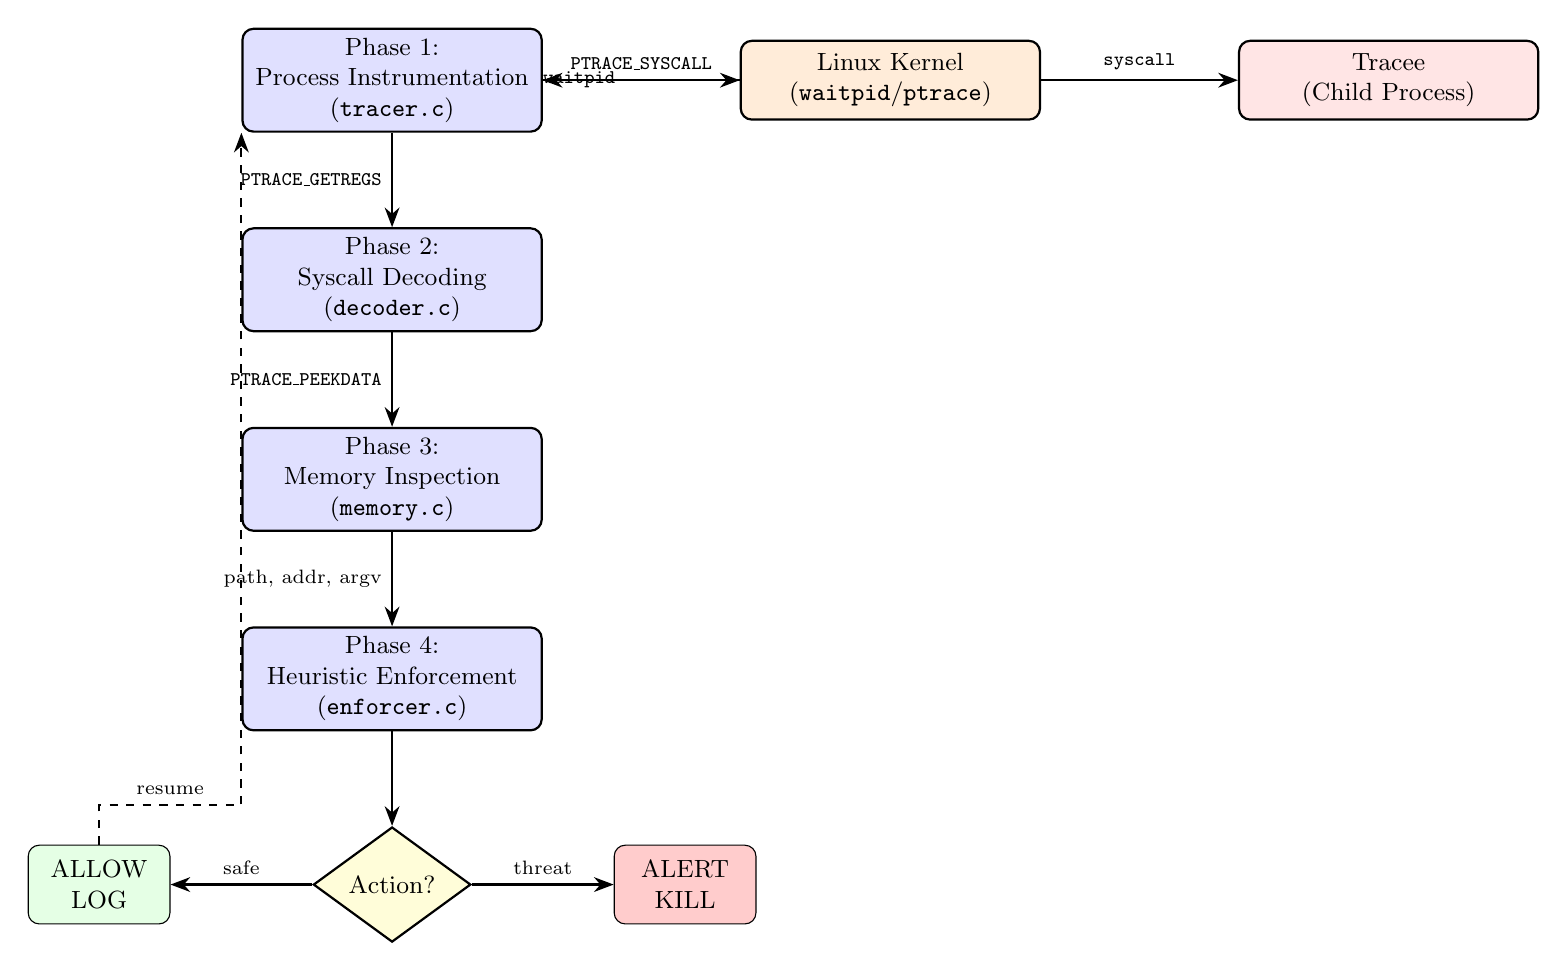
\begin{tikzpicture}[
    node distance=1.5cm and 2cm,
    box/.style={rectangle, draw, rounded corners, minimum width=3.8cm, minimum height=1cm, align=center, font=\small},
    phase/.style={box, fill=blue!12, thick},
    kernel/.style={box, fill=orange!15, thick},
    decision/.style={diamond, draw, thick, fill=yellow!15, minimum width=2cm, minimum height=1cm, align=center, font=\small, inner sep=1pt},
    arrow/.style={-{Stealth[length=2.5mm]}, thick},
]

% Nodes
\node[phase] (tracer) {Phase 1:\\Process Instrumentation\\(\texttt{tracer.c})};
\node[kernel, right=2.5cm of tracer] (kernel) {Linux Kernel\\(\texttt{waitpid}/\texttt{ptrace})};
\node[phase, below=1.2cm of tracer] (decoder) {Phase 2:\\Syscall Decoding\\(\texttt{decoder.c})};
\node[phase, below=1.2cm of decoder] (memory) {Phase 3:\\Memory Inspection\\(\texttt{memory.c})};
\node[phase, below=1.2cm of memory] (enforcer) {Phase 4:\\Heuristic Enforcement\\(\texttt{enforcer.c})};
\node[decision, below=1.2cm of enforcer] (decide) {Action?};

% Right side - child process
\node[box, fill=red!10, thick, right=2.5cm of kernel] (child) {Tracee\\(Child Process)};

% Arrows
\draw[arrow] (tracer) -- node[above, font=\scriptsize]{\texttt{PTRACE\_SYSCALL}} (kernel);
\draw[arrow] (kernel) -- node[above, font=\scriptsize]{\texttt{syscall}} (child);
\draw[arrow] (kernel) -- node[left, font=\scriptsize, xshift=-2mm]{\texttt{waitpid}} (tracer);
\draw[arrow] (tracer) -- node[left, font=\scriptsize]{\texttt{PTRACE\_GETREGS}} (decoder);
\draw[arrow] (decoder) -- node[left, font=\scriptsize]{\texttt{PTRACE\_PEEKDATA}} (memory);
\draw[arrow] (memory) -- node[left, font=\scriptsize]{path, addr, argv} (enforcer);
\draw[arrow] (enforcer) -- (decide);

% Decision outcomes
\node[box, fill=green!10, left=1.8cm of decide, minimum width=1.8cm] (allow) {ALLOW\\LOG};
\node[box, fill=red!20, right=1.8cm of decide, minimum width=1.8cm] (kill) {ALERT\\KILL};

\draw[arrow] (decide) -- node[above, font=\scriptsize]{safe} (allow);
\draw[arrow] (decide) -- node[above, font=\scriptsize]{threat} (kill);

% Resume arrow
\draw[arrow, dashed] (allow.north) -- ++(0, 0.5) -| node[near start, above, font=\scriptsize]{resume} (tracer.south west);

\end{tikzpicture}
\caption{System architecture of Project Overwatch showing the four-phase pipeline}
\label{fig:architecture}
\end{figure}

\section{Detailed Procedures}

The following subsections describe the step-by-step procedures executed in each phase.

\subsection{Phase 1: Process Instrumentation Procedure}

\begin{enumerate}[label=Step \arabic*:]
    \item \texttt{main()} initializes \texttt{tracer\_context\_t} (zeroing all fields, setting defaults).
    \item \texttt{parse\_arguments()} processes CLI flags (\texttt{-e}, \texttt{-p}, \texttt{-d}, \texttt{-q}, \texttt{-h}, \texttt{-v}) and identifies the target program after the \texttt{-{}-} separator.
    \item \texttt{init\_default\_rules()} populates the rule array with 12 detection rules.
    \item \texttt{spawn\_traced\_process()} calls \texttt{fork()}:
    \begin{itemize}
        \item \textbf{Child:} Calls \texttt{ptrace(PTRACE\_TRACEME)}, \texttt{raise(SIGSTOP)}, then \texttt{execvp(target)}.
        \item \textbf{Parent:} Calls \texttt{waitpid(child)} to catch the SIGSTOP, verifies \texttt{WIFSTOPPED}, then sets \texttt{PTRACE\_SETOPTIONS} with \texttt{O\_TRACESYSGOOD | O\_TRACEEXEC}.
    \end{itemize}
    \item \texttt{run\_tracer\_loop()} installs \texttt{SIGINT}/\texttt{SIGTERM} handlers and issues the initial \texttt{PTRACE\_SYSCALL} to resume the child.
\end{enumerate}

\subsection{Phase 2: Syscall Decoding Procedure}

\begin{enumerate}[label=Step \arabic*:]
    \item On each syscall stop, the loop calls \texttt{get\_syscall\_info()}.
    \item \texttt{get\_syscall\_info()} executes \texttt{ptrace(PTRACE\_GETREGS, pid, NULL, \&regs)}.
    \item The function extracts: \texttt{orig\_rax} $\to$ \texttt{syscall\_num}, \texttt{rdi} $\to$ \texttt{arg1}, \texttt{rsi} $\to$ \texttt{arg2}, \texttt{rdx} $\to$ \texttt{arg3}, \texttt{r10} $\to$ \texttt{arg4}, \texttt{r8} $\to$ \texttt{arg5}, \texttt{r9} $\to$ \texttt{arg6}.
    \item \texttt{syscall\_name()} performs a linear search of the 150-entry syscall table.
    \item \texttt{print\_syscall\_info()} classifies the syscall into FILE/NETWORK/PROCESS/SYSTEM and prints color-coded output.
\end{enumerate}

\subsection{Phase 3: Memory Inspection Procedure}

\begin{enumerate}[label=Step \arabic*:]
    \item \texttt{inspect\_syscall\_args()} is called with the \texttt{syscall\_info\_t}.
    \item Based on syscall number, it dispatches to the appropriate reader:
    \begin{itemize}
        \item File syscalls (\texttt{open}, \texttt{stat}, \texttt{unlink}, ...): \texttt{read\_string\_from\_child(pid, arg1, ...)}.
        \item \texttt{openat}-family syscalls: \texttt{read\_string\_from\_child(pid, arg2, ...)}.
        \item \texttt{execve}: \texttt{read\_string\_from\_child(pid, arg1, ...)} + \texttt{read\_argv\_from\_child(pid, arg2, ...)}.
        \item \texttt{connect}/\texttt{bind}: \texttt{read\_sockaddr\_from\_child(pid, arg2, ...)}.
    \end{itemize}
    \item \texttt{read\_string\_from\_child()} iterates: call \texttt{PTRACE\_PEEKDATA} for 8~bytes $\to$ scan bytes for \texttt{'\textbackslash 0'} $\to$ append to buffer $\to$ advance address by 8 $\to$ repeat until null or max length.
    \item \texttt{read\_sockaddr\_from\_child()} reads 16~bytes via \texttt{read\_bytes\_from\_child()}, interprets \texttt{sa\_family} (AF\_INET=2, AF\_INET6=10), manually converts port from network byte order, and formats the IP address string.
\end{enumerate}

\subsection{Phase 4: Heuristic Enforcement Procedure}

\begin{enumerate}[label=Step \arabic*:]
    \item \texttt{evaluate\_syscall()} extracts the file path or network address for the current syscall.
    \item For network syscalls (\texttt{SYS\_CONNECT}): reads the \texttt{sockaddr}, checks the port against the suspicious port list \{4444, 5555, 6666, 31337, 12345, 1234, 8080\}. If matched, returns \texttt{ACTION\_KILL} (enforce mode) or \texttt{ACTION\_ALERT} (passive mode).
    \item For file/exec syscalls: iterates over all enabled rules, checking:
    \begin{itemize}
        \item Does the rule's \texttt{syscall\_num} match? (Or is it \texttt{-1} for ``any''?)
        \item Does the extracted path match the rule's \texttt{path\_pattern} via \texttt{fnmatch()}?
    \end{itemize}
    \item Tracks the highest-severity action across all matching rules.
    \item If enforce mode is active and the maximum threat is $\geq$~HIGH, escalates the action to KILL.
    \item Returns the final action to the interception loop, which dispatches accordingly (increment counters, log, or call \texttt{kill\_traced\_process()}).
\end{enumerate}


% ============================================================================
%                   CHAPTER 6: IMPLEMENTATION DETAILS
% ============================================================================
\chapter{Implementation Details}

This chapter presents the complete implementation of Project Overwatch, organized by module. For each module, the relevant source code is presented alongside detailed, line-by-line explanations of the logic, data structures, and design rationale.

\section{Project Structure}

\begin{table}[H]
\centering
\caption{Source file organization}
\label{tab:structure}
\begin{tabularx}{\textwidth}{l r X}
\toprule
\textbf{File} & \textbf{Lines} & \textbf{Responsibility} \\
\midrule
\texttt{include/watchtower.h} & 207 & Shared header: constants, syscall defines, data structures, prototypes \\
\texttt{src/main.c} & 85 & Entry point: context init, argument parsing, phase orchestration \\
\texttt{src/tracer.c} & 365 & Phase 1: \texttt{fork}/\texttt{ptrace} lifecycle, interception loop, signal handling \\
\texttt{src/decoder.c} & 421 & Phase 2: register reading, 150-entry syscall table, categorization \\
\texttt{src/memory.c} & 373 & Phase 3: cross-process string/struct/argv reading \\
\texttt{src/enforcer.c} & 468 & Phase 4: 12 detection rules, evaluation engine, kill logic \\
\texttt{src/utils.c} & 288 & CLI parsing, color logging, stats, banner \\
\midrule
\textbf{Total} & \textbf{$\sim$2{,}207} & \\
\bottomrule
\end{tabularx}
\end{table}

% ----------------------------------------------------------------------------
\section{Core Data Structures (\texttt{watchtower.h})}
% ----------------------------------------------------------------------------

Before examining the code in each phase, it is essential to understand the data structures that are shared across all modules. These are declared in the shared header \texttt{include/watchtower.h}.

\subsection{Syscall Information Structure}

\begin{lstlisting}[caption={The \texttt{syscall\_info\_t} structure --- captures one intercepted syscall event}, label={lst:sysinfo}]
typedef struct {
    long syscall_num;              /* Syscall number from orig_rax */
    unsigned long long arg1;       /* RDI --- first argument */
    unsigned long long arg2;       /* RSI --- second argument */
    unsigned long long arg3;       /* RDX --- third argument */
    unsigned long long arg4;       /* R10 --- fourth argument */
    unsigned long long arg5;       /* R8  --- fifth argument */
    unsigned long long arg6;       /* R9  --- sixth argument */
    unsigned long long rip;        /* Instruction pointer */
    long return_value;             /* RAX on exit, -ENOSYS on entry */
    bool is_entry;                 /* true = entry stop, false = exit stop */
} syscall_info_t;
\end{lstlisting}

\noindent\textbf{Explanation.}
This structure is the fundamental data unit passed between Phase~2 (decoding) and Phase~4 (enforcement). Each field serves a specific purpose:

\begin{itemize}[leftmargin=2cm]
    \item \textbf{\texttt{syscall\_num}} stores the syscall number read from \texttt{orig\_rax}. The \texttt{long} type is used because the kernel stores syscall numbers as signed long values; invalid or unsupported syscalls return negative numbers.
    \item \textbf{\texttt{arg1}--\texttt{arg6}} correspond directly to the six hardware registers used by the x86\_64 Linux syscall convention (RDI, RSI, RDX, R10, R8, R9). The \texttt{unsigned long long} type matches the 64-bit register width, ensuring no truncation of pointer values or large constants.
    \item \textbf{\texttt{rip}} captures the instruction pointer at the time of the syscall stop. This allows Overwatch to determine \emph{where} in the tracee's code the syscall was issued, which is useful for debugging and could support future code-region-based policies.
    \item \textbf{\texttt{return\_value}} is meaningful only on \emph{exit} stops. On entry, the kernel has already overwritten \texttt{rax} with \texttt{-ENOSYS}; the original syscall number is preserved in \texttt{orig\_rax}.
    \item \textbf{\texttt{is\_entry}} is set by the interception loop's double-stop toggle logic (described in Section~\ref{sec:loop}). It allows downstream modules to know whether they are inspecting a syscall \emph{before} or \emph{after} execution.
\end{itemize}

\subsection{Tracer Context Structure}

\begin{lstlisting}[caption={The \texttt{tracer\_context\_t} structure --- global session state}, label={lst:ctx}]
typedef struct {
    pid_t child_pid;                   /* PID of the traced child process */
    bool is_running;                   /* Loop control flag */
    bool in_syscall;                   /* Double-stop toggle state */
    int log_level;                     /* Current verbosity threshold */
    bool enforce_mode;                 /* true = kill threats; false = log only */
    stats_t stats;                     /* Accumulated session statistics */
    detection_rule_t rules[MAX_RULES]; /* Array of detection rules */
    int rule_count;                    /* Number of active rules */
} tracer_context_t;
\end{lstlisting}

\noindent\textbf{Explanation.}
The \texttt{tracer\_context\_t} is the single ``god object'' that carries all session state through the system. It is allocated on the stack in \texttt{main()} and passed by pointer to every function that needs to read or modify session state. Key design choices:

\begin{itemize}[leftmargin=2cm]
    \item \textbf{\texttt{child\_pid}} is initialized to $-1$ and set to a valid PID only after \texttt{spawn\_traced\_process()} succeeds. All functions check this value before calling \texttt{ptrace}.
    \item \textbf{\texttt{in\_syscall}} implements the double-stop toggle. Because \texttt{PTRACE\_SYSCALL} stops the tracee \emph{twice} per syscall (once on entry, once on exit), this boolean is flipped on each stop. When \texttt{true}, the current stop is an entry; when \texttt{false}, it is an exit. This simple mechanism avoids the need for explicit state machines.
    \item \textbf{\texttt{enforce\_mode}} selects between the two operational modes. In passive mode (\texttt{false}), all threats are logged but the process is never terminated. In enforce mode (\texttt{true}), HIGH and CRITICAL threats are escalated to \texttt{ACTION\_KILL}, and the tracer issues \texttt{PTRACE\_KILL} followed by \texttt{SIGKILL}.
    \item \textbf{\texttt{rules[MAX\_RULES]}} is a fixed-size array (100 slots) of detection rules. This avoids dynamic memory allocation and the associated error-handling complexity. The \texttt{rule\_count} field tracks how many slots are occupied.
    \item \textbf{\texttt{stats}} is an embedded \texttt{stats\_t} structure with seven counters (total syscalls, files accessed, network connections, executions, alerts generated, blocked syscalls, processes killed). These are incremented in real time and printed at session end.
\end{itemize}

\subsection{Detection Rule Structure}

\begin{lstlisting}[caption={The \texttt{detection\_rule\_t} structure --- one heuristic detection rule}, label={lst:ruledef}]
typedef struct {
    const char *name;                /* Short identifier, e.g. "shadow_access" */
    const char *description;         /* Human-readable explanation */
    long syscall_num;                /* Syscall to match, or -1 for any */
    const char *path_pattern;        /* Glob pattern for path matching */
    threat_level_t threat;           /* NONE, LOW, MEDIUM, HIGH, CRITICAL */
    enforcement_action_t action;     /* ALLOW, LOG, ALERT, BLOCK, KILL */
    bool enabled;                    /* Can be toggled at runtime */
} detection_rule_t;
\end{lstlisting}

\noindent\textbf{Explanation.}
Each detection rule encodes a single security policy:

\begin{itemize}[leftmargin=2cm]
    \item \textbf{\texttt{syscall\_num}} restricts the rule to a specific syscall (e.g., \texttt{SYS\_OPEN} for file access rules) or allows matching against any file-related syscall when set to $-1$.
    \item \textbf{\texttt{path\_pattern}} is a POSIX glob pattern passed to \texttt{fnmatch(3)}. The wildcard \texttt{*} matches any sequence of characters within a single path component; the pattern \texttt{/etc/shadow*} therefore matches \texttt{/etc/shadow} and \texttt{/etc/shadow-} but not \texttt{/etc/shadow/subdir}.
    \item \textbf{\texttt{threat}} and \textbf{\texttt{action}} are ordered enumerations. The evaluation engine uses the ordering (\texttt{ALLOW} $<$ \texttt{LOG} $<$ \texttt{ALERT} $<$ \texttt{BLOCK} $<$ \texttt{KILL}) to implement its ``highest-severity-wins'' strategy.
    \item \textbf{\texttt{enabled}} allows individual rules to be toggled without removing them from the array, supporting future hot-reload functionality.
\end{itemize}


% ----------------------------------------------------------------------------
\section{Entry Point and Phase Orchestration (\texttt{main.c})}
% ----------------------------------------------------------------------------

The \texttt{main.c} file is intentionally minimal (85 lines), serving as a thin orchestration layer that initializes the context, parses arguments, and invokes each phase in sequence.

\begin{lstlisting}[caption={\texttt{main()} --- entry point and four-phase orchestration}, label={lst:main}]
int main(int argc, char *argv[]) {
    tracer_context_t ctx;
    int program_idx;
    int exit_code;
    
    /* Step 1: Zero-initialize the entire context */
    init_tracer_context(&ctx);
    
    /* Step 2: Parse CLI flags (-e, -d, -q, etc.) */
    program_idx = parse_arguments(argc, argv, &ctx);
    
    /* Step 3: Validate that a target program was specified */
    if (program_idx < 0 || program_idx >= argc) {
        print_banner();
        fprintf(stderr, "Error: No program specified to trace.\n\n");
        print_usage(argv[0]);
        return 1;
    }
    
    print_banner();
    log_message(LOG_LEVEL_INFO, "Project Overwatch EDR starting...");
    log_message(LOG_LEVEL_INFO, "Target program: %s", argv[program_idx]);
    
    /* Step 4: Load the 12 default detection rules */
    init_default_rules(&ctx);
    
    /* Step 5 (Phase 1): Fork and trace the target */
    ctx.child_pid = spawn_traced_process(argv[program_idx],
                                         &argv[program_idx]);
    if (ctx.child_pid == -1) {
        log_message(LOG_LEVEL_ERROR, "Failed to spawn traced process");
        return 1;
    }
    
    /* Step 6 (Phases 2-4): Enter the interception loop */
    exit_code = run_tracer_loop(&ctx);
    
    /* Step 7: Print session statistics and exit */
    print_stats(&ctx.stats);
    return exit_code;
}
\end{lstlisting}

\noindent\textbf{Line-by-line explanation:}

\begin{enumerate}[leftmargin=1.5cm]
    \item[\textbf{Lines 2--4:}] Three local variables are declared: a \texttt{tracer\_context\_t} on the stack (no heap allocation), an index into \texttt{argv} pointing to the first non-option argument, and the eventual exit code.

    \item[\textbf{Line 7:}] \texttt{init\_tracer\_context(\&ctx)} calls \texttt{memset} to zero the entire structure, then sets \texttt{child\_pid} to $-1$ (invalid), \texttt{enforce\_mode} to \texttt{false} (passive by default), and all statistic counters to zero. This ensures deterministic initial state regardless of stack contents.

    \item[\textbf{Line 10:}] \texttt{parse\_arguments()} walks \texttt{argv[1..n]} looking for flags. The \texttt{-{}-} separator marks the boundary between Overwatch's options and the target program's command line. The function returns the index of the first argument \emph{after} the separator (or the first non-flag argument if \texttt{-{}-} is absent). If \texttt{-e} is found, \texttt{ctx.enforce\_mode} is set to \texttt{true}; if \texttt{-d} is found, the global log level is lowered to \texttt{LOG\_LEVEL\_DEBUG}.

    \item[\textbf{Lines 13--17:}] If no target program was specified (e.g., the user ran \texttt{./overwatch -e} without naming a program), the banner and usage instructions are printed and the program exits with code 1.

    \item[\textbf{Line 24:}] \texttt{init\_default\_rules(\&ctx)} populates \texttt{ctx.rules[0..11]} with 12 hardcoded detection rules (detailed in Section~\ref{sec:rules}) and sets \texttt{ctx.rule\_count = 12}.

    \item[\textbf{Lines 27--28:}] \texttt{spawn\_traced\_process()} is the Phase~1 entry point. It calls \texttt{fork()}, sets up ptrace in the child, and waits for the child to stop. The returned PID is stored in \texttt{ctx.child\_pid}. The \texttt{\&argv[program\_idx]} expression passes the remaining command-line arguments as the target's \texttt{argv} array.

    \item[\textbf{Line 34:}] \texttt{run\_tracer\_loop(\&ctx)} is the heart of the system. It enters the TRAP--PAUSE--INSPECT--DECIDE cycle (Phases~2--4) and does not return until the child exits, is killed, or the user presses Ctrl+C. The exit code of the child is returned.

    \item[\textbf{Line 37:}] \texttt{print\_stats()} outputs the seven session counters in a formatted, color-coded table.
\end{enumerate}


% ----------------------------------------------------------------------------
\section{Phase 1: Process Instrumentation (\texttt{tracer.c})}
% ----------------------------------------------------------------------------

The instrumentation module (365 lines) is the foundation of the entire system. It manages the ptrace lifecycle---spawning the child, configuring tracing options, and implementing the main interception loop.

\subsection{Signal Handler for Graceful Shutdown}

\begin{lstlisting}[caption={Signal handler and global shutdown flag}, label={lst:sighandler}]
static volatile sig_atomic_t g_shutdown_requested = 0;

static void signal_handler(int sig) {
    if (sig == SIGINT || sig == SIGTERM) {
        g_shutdown_requested = 1;
    }
}
\end{lstlisting}

\noindent\textbf{Explanation.}
The \texttt{g\_shutdown\_requested} variable is declared \texttt{volatile sig\_atomic\_t}---the only C type guaranteed to be safely written from inside a signal handler. The \texttt{volatile} qualifier prevents the compiler from optimizing away repeated reads of the flag in the interception loop. When the user presses Ctrl+C, the operating system delivers \texttt{SIGINT} to the tracer process. The handler sets the flag to 1; the interception loop checks this flag on every iteration (see Listing~\ref{lst:loop}) and performs a clean \texttt{PTRACE\_DETACH} when it detects the flag. This two-step design avoids calling non-async-signal-safe functions (such as \texttt{printf} or \texttt{ptrace}) from within the signal handler itself.

\subsection{Spawning a Traced Process}

\begin{lstlisting}[caption={Complete \texttt{spawn\_traced\_process()} function}, label={lst:spawn}]
pid_t spawn_traced_process(const char *program, char *const argv[]) {
    pid_t child_pid;
    
    child_pid = fork();
    
    if (child_pid == -1) {
        log_message(LOG_LEVEL_ERROR, "fork() failed: %s", strerror(errno));
        return -1;
    }
    
    if (child_pid == 0) {
        /* ============= CHILD PROCESS (Tracee) ============= */
        
        /* (a) Request tracing by parent */
        if (ptrace(PTRACE_TRACEME, 0, NULL, NULL) == -1) {
            fprintf(stderr, "[CHILD] PTRACE_TRACEME failed: %s\n",
                    strerror(errno));
            _exit(1);
        }
        
        /* (b) Stop ourselves to synchronize with parent */
        raise(SIGSTOP);
        
        /* (c) Replace our memory image with the target program */
        execvp(program, argv);
        
        /* (d) If we reach here, exec failed */
        fprintf(stderr, "[CHILD] execvp(%s) failed: %s\n",
                program, strerror(errno));
        _exit(1);
    }
    
    /* ============= PARENT PROCESS (Tracer) ============= */
    int status;
    
    /* (e) Wait for child to stop at SIGSTOP */
    waitpid(child_pid, &status, 0);
    
    if (!WIFSTOPPED(status)) {
        log_message(LOG_LEVEL_ERROR, "Child did not stop as expected");
        return -1;
    }
    
    /* (f) Configure ptrace options */
    ptrace(PTRACE_SETOPTIONS, child_pid, 0,
           PTRACE_O_TRACESYSGOOD | PTRACE_O_TRACEEXEC);
    
    return child_pid;
}
\end{lstlisting}

\noindent\textbf{Detailed explanation:}

\begin{enumerate}[leftmargin=1.5cm]
    \item[\textbf{Line 4} (\texttt{fork}):] The \texttt{fork()} system call creates a new process by duplicating the calling process. After \texttt{fork()}, two processes exist with identical memory images: the parent (tracer) receives the child's PID as the return value, and the child receives 0. Error is indicated by $-1$.

    \item[\textbf{Line 15} (\texttt{PTRACE\_TRACEME}):] The child calls \texttt{ptrace(PTRACE\_TRACEME, 0, NULL, NULL)} to volunteer itself for tracing. This does two things: (1) it marks the process as ``being traced'' in the kernel's task structure, and (2) it designates the parent process as the tracer. After this call, any signal delivered to the child will first cause the child to \emph{stop}, and the parent to be notified via \texttt{waitpid()}. This call must occur \emph{before} \texttt{execvp}, because \texttt{exec} generates a \texttt{SIGTRAP} that would be uncaught otherwise.

    \item[\textbf{Line 22} (\texttt{raise(SIGSTOP)}):] The child sends itself a \texttt{SIGSTOP} signal, which suspends execution. This is a critical synchronization point: the parent is already blocked in \texttt{waitpid()} (line 38), waiting for the child to stop. Without this explicit stop, there is a race condition---the child might call \texttt{execvp} before the parent has configured ptrace options, causing the system to miss the initial \texttt{SIGTRAP} from \texttt{exec}.

    \item[\textbf{Line 25} (\texttt{execvp}):] \texttt{execvp(program, argv)} replaces the child's entire memory image (code, data, stack, heap) with the target program. The ``v'' means arguments are passed as a vector (\texttt{argv} array); the ``p'' means the system searches \texttt{\$PATH} if \texttt{program} contains no slashes. After a successful \texttt{exec}, \emph{none of the child's original code remains in memory}---execution begins at the target program's entry point. The PID, file descriptors, and ptrace status are preserved across \texttt{exec}.

    \item[\textbf{Line 30} (\texttt{\_exit(1)}):] If \texttt{execvp} returns, it has failed (e.g., file not found, permission denied). The child calls \texttt{\_exit(1)}---not \texttt{exit(1)}---because \texttt{\_exit} skips \texttt{atexit} handlers and stdio buffer flushing, which is critical after \texttt{fork} to avoid corrupting the parent's buffered output.

    \item[\textbf{Line 38} (\texttt{waitpid}):] The parent blocks until the child changes state. The \texttt{WIFSTOPPED(status)} macro returns true if the child was stopped by a signal (in this case, the \texttt{SIGSTOP} raised by the child on line~22).

    \item[\textbf{Lines 46--47} (\texttt{PTRACE\_SETOPTIONS}):] Two options are configured:
    \begin{itemize}
        \item \texttt{PTRACE\_O\_TRACESYSGOOD}: Modifies syscall-stop signals by setting bit~7 of the signal number, producing \texttt{SIGTRAP | 0x80} (decimal 133) instead of plain \texttt{SIGTRAP} (decimal 5). This is critical because it allows the interception loop to distinguish \emph{syscall stops} from other \texttt{SIGTRAP} events (breakpoints, single-step traps, \texttt{exec} notifications). Without this option, every \texttt{SIGTRAP} would be ambiguous.
        \item \texttt{PTRACE\_O\_TRACEEXEC}: Causes the kernel to send a \texttt{PTRACE\_EVENT\_EXEC} notification when the tracee calls \texttt{exec}. This allows Overwatch to detect process replacement.
    \end{itemize}
\end{enumerate}

\subsection{The Interception Loop}
\label{sec:loop}

The \texttt{run\_tracer\_loop()} function implements the core TRAP--PAUSE--INSPECT--DECIDE cycle. This is the largest function in the project and the single most critical piece of logic:

\begin{lstlisting}[caption={Interception loop (simplified from \texttt{run\_tracer\_loop()})}, label={lst:loop}]
/* Install signal handlers for graceful shutdown */
struct sigaction sa;
sa.sa_handler = signal_handler;
sigemptyset(&sa.sa_mask);
sa.sa_flags = 0;
sigaction(SIGINT, &sa, NULL);
sigaction(SIGTERM, &sa, NULL);

ctx->is_running = 1;
ctx->in_syscall = 0;  /* Start outside a syscall */

/* Resume the child, stopping at the next syscall */
ptrace(PTRACE_SYSCALL, ctx->child_pid, NULL, NULL);

while (ctx->is_running && !g_shutdown_requested) {
    /* STEP 1: Wait for child to stop */
    pid_t result = waitpid(ctx->child_pid, &status, 0);
    
    if (result == -1) {
        if (errno == EINTR) continue;   /* Interrupted by signal */
        break;                          /* Fatal error */
    }
    
    /* STEP 2: Check termination */
    if (WIFEXITED(status))   { ctx->is_running = 0; break; }
    if (WIFSIGNALED(status)) { ctx->is_running = 0; break; }
    
    if (WIFSTOPPED(status)) {
        int stop_sig = WSTOPSIG(status);
        
        if (stop_sig == (SIGTRAP | 0x80) || stop_sig == SIGTRAP) {
            /* --- SYSCALL STOP --- */
            get_syscall_info(ctx->child_pid, &sysinfo);
            ctx->in_syscall = !ctx->in_syscall;  /* Toggle */
            sysinfo.is_entry = ctx->in_syscall;
            
            if (sysinfo.is_entry) {
                /* ENTRY: Inspect BEFORE the kernel executes */
                ctx->stats.total_syscalls++;
                print_syscall_info(&sysinfo);
                action = evaluate_syscall(ctx, &sysinfo);
                
                if (action == ACTION_KILL) {
                    kill_traced_process(ctx->child_pid,
                                       "Malicious syscall detected");
                    ctx->stats.processes_killed++;
                    ctx->is_running = 0;
                    break;
                } else if (action == ACTION_BLOCK) {
                    ctx->stats.blocked_syscalls++;
                } else if (action == ACTION_ALERT) {
                    ctx->stats.alerts_generated++;
                }
            }
            /* Resume to next syscall boundary */
            ptrace(PTRACE_SYSCALL, ctx->child_pid, NULL, NULL);
            
        } else {
            /* --- NON-SYSCALL SIGNAL: relay to child --- */
            ptrace(PTRACE_SYSCALL, ctx->child_pid, NULL,
                   (void*)(long)stop_sig);
        }
    }
}

/* Cleanup on shutdown */
if (g_shutdown_requested && ctx->is_running)
    detach_from_process(ctx->child_pid);
\end{lstlisting}

\noindent\textbf{Detailed block-by-block explanation:}

\begin{enumerate}[leftmargin=1.5cm]
    \item[\textbf{Lines 1--6} (Signal setup):] The handler from Listing~\ref{lst:sighandler} is installed using \texttt{sigaction} (not the older \texttt{signal()} function, which has undefined behavior in multi-threaded contexts). \texttt{sigemptyset(\&sa.sa\_mask)} ensures no signals are blocked while the handler runs. Two signals are registered: \texttt{SIGINT} (Ctrl+C) and \texttt{SIGTERM} (\texttt{kill} command).

    \item[\textbf{Lines 9--10} (State initialization):] The loop control flag \texttt{is\_running} is set to true, and \texttt{in\_syscall} is initialized to \texttt{false} (0), indicating we start \emph{outside} a syscall.

    \item[\textbf{Line 13} (Initial resume):] The first \texttt{PTRACE\_SYSCALL} resumes the child (which is currently stopped at the \texttt{SIGSTOP} from the spawn function). The child will execute until it hits its first syscall, at which point the kernel stops it again and \texttt{waitpid} returns.

    \item[\textbf{Line 17} (\texttt{waitpid}):] The parent blocks until the child changes state. The return value is the child's PID on success, or $-1$ on error. If the call was interrupted by a signal (\texttt{errno == EINTR}), the loop restarts---this handles the case where the user presses Ctrl+C while \texttt{waitpid} is blocking.

    \item[\textbf{Lines 25--26} (Termination checks):] Two macros are checked:
    \begin{itemize}
        \item \texttt{WIFEXITED(status)}: True if the child called \texttt{exit()} or returned from \texttt{main()}. \texttt{WEXITSTATUS(status)} extracts the exit code.
        \item \texttt{WIFSIGNALED(status)}: True if the child was killed by a signal (e.g., \texttt{SIGSEGV}, \texttt{SIGKILL}). \texttt{WTERMSIG(status)} extracts the signal number.
    \end{itemize}

    \item[\textbf{Line 31} (Syscall detection):] The key test: if the stop signal is \texttt{SIGTRAP | 0x80} (decimal 133), this is a syscall stop generated by \texttt{PTRACE\_SYSCALL} with the \texttt{TRACESYSGOOD} option. The fallback to plain \texttt{SIGTRAP} handles the (unlikely) case where \texttt{PTRACE\_SETOPTIONS} failed during spawn.

    \item[\textbf{Lines 33--35} (Double-stop toggle):] \texttt{get\_syscall\_info()} reads the CPU registers (Phase~2). The \texttt{in\_syscall} flag is then toggled: \texttt{false} $\to$ \texttt{true} means entry, \texttt{true} $\to$ \texttt{false} means exit. This toggle-based approach works because \texttt{PTRACE\_SYSCALL} generates exactly one stop per syscall boundary, and stops alternate strictly between entry and exit for a given process.

    \item[\textbf{Lines 38--53} (Entry processing):] On entry, the function:
    \begin{enumerate}[label=(\alph*)]
        \item Increments \texttt{total\_syscalls},
        \item Calls \texttt{print\_syscall\_info()} (Phase~2) to produce color-coded terminal output,
        \item Calls \texttt{evaluate\_syscall()} (Phase~4) which internally invokes Phase~3 memory inspection,
        \item Dispatches the returned action: \texttt{ACTION\_KILL} terminates the child via \texttt{kill\_traced\_process()}, \texttt{ACTION\_BLOCK} increments the block counter, and \texttt{ACTION\_ALERT} increments the alert counter.
    \end{enumerate}

    \item[\textbf{Line 55} (Resume):] \texttt{PTRACE\_SYSCALL} with a \texttt{NULL} fourth argument resumes the child and requests that it be stopped at the next syscall boundary (either the exit of the current syscall, or the entry of the next one).

    \item[\textbf{Lines 58--60} (Signal relay):] If the child was stopped by a signal other than a syscall trap (e.g., \texttt{SIGCHLD}, \texttt{SIGALRM}, \texttt{SIGPIPE}), the signal is \emph{forwarded} to the child by passing its number as the fourth argument to \texttt{PTRACE\_SYSCALL}. This is critical: if the tracer suppresses signals (by passing 0), any program that relies on signal delivery for normal operation (timers, child-process notification, pipe handling) will malfunction.

    \item[\textbf{Lines 64--65} (Graceful detach):] If the loop exits because Ctrl+C was pressed (not because the child terminated), the tracer calls \texttt{PTRACE\_DETACH}. This releases the child process from tracing and allows it to continue executing normally.
\end{enumerate}


% ----------------------------------------------------------------------------
\section{Phase 2: Syscall Decoding (\texttt{decoder.c})}
% ----------------------------------------------------------------------------

The decoder module (421 lines) translates raw CPU register values into human-readable syscall events.

\subsection{Register Extraction}

The \texttt{get\_syscall\_info()} function uses a single \texttt{PTRACE\_GETREGS} call to read all 27 CPU registers into a \texttt{struct user\_regs\_struct} (defined in \texttt{<sys/user.h>}). Overwatch extracts the 9 fields relevant to syscall analysis:

\begin{lstlisting}[caption={Register extraction in \texttt{get\_syscall\_info()}}, label={lst:regs}]
int get_syscall_info(pid_t pid, syscall_info_t *info) {
    struct user_regs_struct regs;
    
    /* Read all registers in a single ptrace call */
    if (ptrace(PTRACE_GETREGS, pid, NULL, &regs) == -1) {
        log_message(LOG_LEVEL_ERROR, "PTRACE_GETREGS failed: %s",
                    strerror(errno));
        return -1;
    }
    
    /* Map registers to syscall_info_t fields */
    info->syscall_num  = regs.orig_rax;  /* Preserved syscall number */
    info->arg1         = regs.rdi;       /* 1st argument */
    info->arg2         = regs.rsi;       /* 2nd argument */
    info->arg3         = regs.rdx;       /* 3rd argument */
    info->arg4         = regs.r10;       /* 4th argument */
    info->arg5         = regs.r8;        /* 5th argument */
    info->arg6         = regs.r9;        /* 6th argument */
    info->rip          = regs.rip;       /* Instruction pointer */
    info->return_value = regs.rax;       /* Return value (exit only) */
    
    return 0;
}
\end{lstlisting}

\noindent\textbf{Detailed explanation:}

\begin{itemize}[leftmargin=2cm]
    \item \textbf{\texttt{PTRACE\_GETREGS}} reads the entire general-purpose register set in a single system call, avoiding the overhead of 9 separate \texttt{PTRACE\_PEEKUSER} calls. The kernel copies the registers from the tracee's saved register area (stored on the kernel stack when the process entered the syscall) into the \texttt{regs} structure in the tracer's address space.

    \item \textbf{\texttt{regs.orig\_rax} vs.\ \texttt{regs.rax}}: This distinction is one of the most subtle aspects of ptrace on x86\_64. When a user-space program executes the \texttt{syscall} instruction, the CPU places the syscall number in \texttt{RAX}. The kernel then:
    \begin{enumerate}
        \item Saves the original \texttt{RAX} value in the \texttt{orig\_rax} field of the task's register save area.
        \item Overwrites \texttt{RAX} with \texttt{-ENOSYS} (``Function not implemented'').
        \item Dispatches the syscall using the saved \texttt{orig\_rax} value.
        \item On return, writes the syscall's return value into \texttt{RAX}.
    \end{enumerate}
    Therefore, on a syscall \emph{entry} stop, \texttt{regs.rax} contains \texttt{-ENOSYS} (useless), while \texttt{regs.orig\_rax} contains the actual syscall number. On an \emph{exit} stop, \texttt{regs.rax} contains the return value, and \texttt{regs.orig\_rax} still holds the syscall number.

    \item \textbf{Register-to-argument mapping} follows the System V AMD64 ABI convention used by all x86\_64 Linux systems. The first six integer/pointer arguments to a syscall are passed in registers RDI, RSI, RDX, R10, R8, R9 (note: R10 replaces RCX for syscalls because the \texttt{syscall} instruction clobbers RCX). This differs from the \emph{function call} convention, which uses RCX for the fourth argument.
\end{itemize}

\subsection{Syscall Name Table}

\begin{lstlisting}[caption={Syscall table structure and sample entries}, label={lst:table}]
typedef struct {
    long number;
    const char *name;
    const char *description;
} syscall_entry_t;

static const syscall_entry_t syscall_table[] = {
    {  0,  "read",     "Read from file descriptor"     },
    {  1,  "write",    "Write to file descriptor"      },
    {  2,  "open",     "Open file"                     },
    {  3,  "close",    "Close file descriptor"         },
    /* ... 150+ entries covering all common syscalls ... */
    { 59,  "execve",   "Execute program"               },
    { 41,  "socket",   "Create socket"                 },
    { 42,  "connect",  "Connect to remote socket"      },
    { 257, "openat",   "Open file relative to directory"},
    { -1,  NULL,       NULL } /* Sentinel */
};
\end{lstlisting}

\noindent\textbf{Explanation.}
The table is a statically allocated array of \texttt{syscall\_entry\_t} records, terminated by a sentinel entry with \texttt{number = -1} and \texttt{name = NULL}. The \texttt{const} qualifier places the array in the read-only data segment, and the \texttt{static} linkage restricts visibility to \texttt{decoder.c}.

Name lookup is performed by \texttt{syscall\_name()}, which iterates linearly through the array until a matching number is found or the sentinel is reached. Although $O(n)$, this is negligible in practice: the table has approximately 150 entries, and the function is called at most once per syscall stop (typically $<$1~$\mu$s per lookup on modern CPUs).

\subsection{Syscall Categorization}

Three \texttt{static} helper functions classify syscalls into categories using \texttt{switch} statements:

\begin{lstlisting}[caption={Syscall categorization functions}, label={lst:category}]
static int is_file_syscall(long syscall_num) {
    switch (syscall_num) {
        case SYS_OPEN: case SYS_OPENAT: case SYS_CREAT:
        case SYS_READ: case SYS_WRITE:  case SYS_CLOSE:
        case SYS_STAT: case SYS_FSTAT:  case SYS_LSTAT:
        case SYS_ACCESS: case SYS_RENAME: case SYS_MKDIR:
        case SYS_RMDIR: case SYS_UNLINK: case SYS_CHMOD:
        case SYS_CHOWN: case SYS_LINK:   case SYS_UNLINKAT:
        case SYS_RENAMEAT: case SYS_MKDIRAT:
            return 1;
        default: return 0;
    }
}

static int is_network_syscall(long syscall_num) {
    switch (syscall_num) {
        case SYS_SOCKET: case SYS_CONNECT: case SYS_ACCEPT:
        case SYS_SENDTO: case SYS_RECVFROM:
        case SYS_BIND:   case SYS_LISTEN:
            return 1;
        default: return 0;
    }
}

static int is_process_syscall(long syscall_num) {
    switch (syscall_num) {
        case SYS_FORK: case SYS_VFORK: case SYS_CLONE:
        case SYS_EXECVE: case SYS_EXECVEAT:
        case SYS_KILL: case SYS_EXIT:
            return 1;
        default: return 0;
    }
}
\end{lstlisting}

\noindent\textbf{Explanation.}
The categorization system partitions the Linux syscall space into four groups:

\begin{itemize}[leftmargin=2cm]
    \item \textbf{FILE} (20 syscalls): All operations that create, open, read, write, delete, rename, or modify metadata of filesystem objects. Both legacy syscalls (\texttt{open}) and their modern \texttt{*at} variants (\texttt{openat}) are included.
    \item \textbf{NETWORK} (7 syscalls): Socket creation, connection, and data transfer operations. These are the syscalls most relevant to detecting command-and-control communication and data exfiltration.
    \item \textbf{PROCESS} (7 syscalls): Process creation (\texttt{fork}, \texttt{clone}), program execution (\texttt{execve}), and termination (\texttt{exit}, \texttt{kill}). These map directly to MITRE ATT\&CK execution and persistence techniques.
    \item \textbf{SYSTEM} (all remaining): Memory management (\texttt{mmap}, \texttt{brk}), signal handling, time operations, and other infrastructure syscalls.
\end{itemize}

\noindent Each category is assigned a distinct ANSI color code in \texttt{print\_syscall\_info()}: bold red for PROCESS (highest threat), bold magenta for NETWORK, bold yellow for FILE, and bold cyan for SYSTEM. The color-coding provides an immediate visual summary of the tracee's behavior profile.


% ----------------------------------------------------------------------------
\section{Phase 3: Memory Inspection (\texttt{memory.c})}
% ----------------------------------------------------------------------------

The memory inspection module (373 lines) implements the most technically challenging aspect of the system: reading data from the tracee's virtual address space across the process boundary.

\subsection{Word-Level Memory Read Primitive}

\begin{lstlisting}[caption={The \texttt{peek\_word()} helper --- reading 8 bytes from the tracee}, label={lst:peek}]
static int peek_word(pid_t pid, unsigned long addr, unsigned long *word) {
    errno = 0;
    *word = ptrace(PTRACE_PEEKDATA, pid, (void*)addr, NULL);
    
    if (*word == (unsigned long)-1 && errno != 0) {
        return -1;
    }
    return 0;
}
\end{lstlisting}

\noindent\textbf{Explanation.}
\texttt{PTRACE\_PEEKDATA} is unique among ptrace requests: it returns the read data \emph{directly} as its return value (rather than through a pointer parameter). The problem is that a valid data word might coincidentally equal \texttt{(unsigned long)-1} (all bits set). The standard idiom is:
\begin{enumerate}
    \item Clear \texttt{errno} to zero \emph{before} the call.
    \item After the call, check if the return value is $-1$ \emph{and} \texttt{errno} is non-zero.
    \item If \texttt{errno} is still zero, the data is valid (it just happens to be \texttt{0xFFFFFFFFFFFFFFFF}).
\end{enumerate}
This function reads exactly 8 bytes (one x86\_64 machine word) from address \texttt{addr} in the tracee's virtual address space.

\subsection{String Reconstruction}

\begin{lstlisting}[caption={Cross-process string reading (\texttt{read\_string\_from\_child()})}, label={lst:string}]
int read_string_from_child(pid_t pid, unsigned long addr,
                           char *buffer, size_t max_len) {
    size_t bytes_read = 0;
    unsigned long word;
    char *word_bytes;
    
    if (addr == 0) {                        /* NULL pointer guard */
        buffer[0] = '\0';
        return 0;
    }
    if (max_len < WORD_SIZE + 1) {          /* Buffer too small */
        return -1;
    }
    max_len--;                              /* Reserve for '\0' */
    
    while (bytes_read < max_len) {
        if (peek_word(pid, addr, &word) == -1)
            break;                          /* Read error */
        
        word_bytes = (char*)&word;
        
        for (int i = 0; i < WORD_SIZE && bytes_read < max_len; i++) {
            buffer[bytes_read] = word_bytes[i];
            if (word_bytes[i] == '\0')      /* Found terminator */
                return bytes_read;
            bytes_read++;
        }
        addr += WORD_SIZE;                  /* Advance to next word */
    }
    
    buffer[bytes_read] = '\0';              /* Truncate safely */
    return bytes_read;
}
\end{lstlisting}

\noindent\textbf{Line-by-line explanation:}

\begin{enumerate}[leftmargin=1.5cm]
    \item[\textbf{Lines 7--9} (NULL guard):] When a syscall argument is a null pointer (e.g., \texttt{open(NULL, ...)}), the function returns an empty string immediately rather than attempting to read from address 0, which would cause a ptrace error.

    \item[\textbf{Lines 11--13} (Size check):] The buffer must be at least $\texttt{WORD\_SIZE} + 1 = 9$ bytes. This ensures that even a single \texttt{PTRACE\_PEEKDATA} read can be stored with a null terminator. One byte is reserved for the terminator by decrementing \texttt{max\_len}.

    \item[\textbf{Lines 16--17} (Word read):] Each iteration calls \texttt{peek\_word()} to read 8 bytes from the tracee. If the read fails (e.g., the address is unmapped), the loop terminates and returns whatever was collected so far.

    \item[\textbf{Lines 20--26} (Byte scanning):] The 8-byte word is treated as a character array. Each byte is copied into the output buffer, and the inner loop checks for a null terminator (\texttt{'\textbackslash 0'}). If found, the function returns immediately with the string length. This null-scanning is necessary because C strings are variable-length; the function cannot know in advance how many bytes constitute the string.

    \item[\textbf{Line 28} (Address advancement):] After processing all 8 bytes of a word, the address is incremented by \texttt{WORD\_SIZE} (8) to move to the next aligned word in the tracee's memory.

    \item[\textbf{Line 31} (Truncation):] If the string exceeds \texttt{max\_len}, the function null-terminates at the boundary and returns the truncated length. This prevents buffer overflows while providing as much data as possible.
\end{enumerate}

\subsection{Socket Address Decoding}

For network syscalls such as \texttt{connect()}, the second argument (\texttt{RSI}) is a pointer to a \texttt{sockaddr} structure in the tracee's memory. The \texttt{read\_sockaddr\_from\_child()} function reads and interprets this structure:

\begin{lstlisting}[caption={Socket address decoding from tracee memory}, label={lst:sockaddr}]
int read_sockaddr_from_child(pid_t pid, unsigned long addr,
                             char *out_addr, size_t addr_len,
                             int *out_port) {
    /* Local replica of sockaddr_in (avoids header dependency) */
    struct {
        unsigned short family;  /* AF_INET=2, AF_INET6=10 */
        unsigned short port;    /* Network byte order */
        unsigned int   addr;    /* IPv4 address (4 bytes) */
        char zero[8];           /* Padding */
    } sa;
    
    /* Read 16 bytes from the tracee's memory */
    if ((size_t)read_bytes_from_child(pid, addr, &sa, sizeof(sa))
        < sizeof(sa))
        return -1;
    
    if (sa.family == 2) {  /* AF_INET (IPv4) */
        /* Convert port from network byte order (big-endian) to host */
        unsigned short port = ((sa.port & 0xFF) << 8)
                            | ((sa.port >> 8) & 0xFF);
        unsigned int ip = sa.addr;
        
        /* Format IPv4 address as dotted-decimal */
        snprintf(out_addr, addr_len, "%u.%u.%u.%u",
                  ip & 0xFF,
                 (ip >> 8)  & 0xFF,
                 (ip >> 16) & 0xFF,
                 (ip >> 24) & 0xFF);
        *out_port = port;
        return 0;
    } else if (sa.family == 10) {  /* AF_INET6 */
        snprintf(out_addr, addr_len, "[IPv6]");
        *out_port = ((sa.port & 0xFF) << 8) | ((sa.port >> 8) & 0xFF);
        return 0;
    }
    return -1;  /* Unknown address family */
}
\end{lstlisting}

\noindent\textbf{Detailed explanation:}

\begin{itemize}[leftmargin=2cm]
    \item \textbf{Lines 5--10 (Local structure):} Instead of including \texttt{<netinet/in.h>}, the function defines a local anonymous structure that mirrors the layout of \texttt{struct sockaddr\_in}. This avoids header conflicts and makes the byte layout explicit: 2 bytes for the address family, 2 bytes for the port in network byte order, 4 bytes for the IPv4 address, and 8 bytes of padding to fill the 16-byte \texttt{sockaddr} structure.

    \item \textbf{Lines 13--15 (\texttt{read\_bytes\_from\_child}):} This helper function (not shown here) reads an arbitrary number of bytes from the tracee, handling word-alignment and partial-word reads internally. The 16 bytes constitute the entire \texttt{sockaddr\_in} structure.

    \item \textbf{Lines 19--20 (Byte-order conversion):} Network protocols use big-endian byte order, while x86\_64 is little-endian. The manual byte swap (\texttt{((port \& 0xFF) << 8) | ((port >> 8) \& 0xFF)}) is used instead of \texttt{ntohs()} to avoid additional header dependencies. The effect is identical: the high byte and low byte of the 16-bit port number are exchanged.

    \item \textbf{Lines 25--28 (IP formatting):} The 32-bit IPv4 address is stored in network byte order (big-endian). On little-endian x86\_64, the first byte at the lowest memory address is the least-significant byte when loaded into a register. The masking and shifting operations extract each octet: \texttt{ip \& 0xFF} gives the first octet (e.g., 127), \texttt{(ip >> 8) \& 0xFF} gives the second (e.g., 0), and so on.

    \item \textbf{Lines 31--34 (IPv6):} Full IPv6 address parsing is not implemented. The function returns a placeholder string \texttt{[IPv6]} with the decoded port number. This is a known limitation documented in Chapter~8.
\end{itemize}

\subsection{Argument Array Reading}

\begin{lstlisting}[caption={\texttt{read\_argv\_from\_child()} --- two-level pointer dereferencing}, label={lst:argv}]
int read_argv_from_child(pid_t pid, unsigned long argv_addr,
                         char args[][MAX_STRING_LENGTH], int max_args) {
    unsigned long ptr;
    int argc = 0;
    
    if (argv_addr == 0) return 0;       /* NULL argv */
    
    while (argc < max_args) {
        /* Step 1: Read the pointer at argv[argc] */
        if (peek_word(pid, argv_addr + (argc * WORD_SIZE), &ptr) == -1)
            break;
        
        if (ptr == 0) break;            /* NULL terminator */
        
        /* Step 2: Follow the pointer to read the string */
        if (read_string_from_child(pid, ptr, args[argc],
                                   MAX_STRING_LENGTH) < 0)
            strcpy(args[argc], "<error>");
        
        argc++;
    }
    return argc;
}
\end{lstlisting}

\noindent\textbf{Explanation.}
This function implements a two-level memory traversal required to read \texttt{execve()} arguments:

\begin{enumerate}
    \item \textbf{Level 1 --- Pointer array:} The \texttt{argv} parameter of \texttt{execve} is a pointer to an array of \texttt{char*} pointers in the tracee's memory. Each pointer is 8 bytes (one word on x86\_64). The function reads the $n$-th pointer from address \texttt{argv\_addr + (n $\times$ 8)}.

    \item \textbf{Level 2 --- String data:} Each pointer in the array points to a null-terminated string elsewhere in the tracee's memory. The function calls \texttt{read\_string\_from\_child()} to follow this pointer and reconstruct the string.

    \item \textbf{Termination:} The array is terminated by a \texttt{NULL} pointer (value 0). When \texttt{peek\_word} returns 0, the function stops iterating.
\end{enumerate}

\noindent This two-level indirection pattern (pointer array $\to$ individual strings) is the same pattern used by the C runtime to construct the \texttt{argv} array passed to \texttt{main()}.


% ----------------------------------------------------------------------------
\section{Phase 4: Heuristic Enforcement (\texttt{enforcer.c})}
\label{sec:rules}
% ----------------------------------------------------------------------------

The enforcement module (468 lines) implements the detection engine: 12 rules, a multi-rule evaluation engine, and the process termination logic.

\subsection{Detection Rules}

The rule engine maintains an array of up to \texttt{MAX\_RULES} (100) \texttt{detection\_rule\_t} structures, initialized by \texttt{init\_default\_rules()}. Each rule is specified using C99 designated initializers:

\begin{lstlisting}[caption={Sample rule initialization (2 of 12 rules shown)}, label={lst:ruleinit}]
/* Rule 1: Block reading the shadow password file */
ctx->rules[idx++] = (detection_rule_t){
    .name        = "shadow_access",
    .description = "Attempt to read /etc/shadow (password hashes)",
    .syscall_num = SYS_OPEN,
    .path_pattern = "/etc/shadow*",
    .threat      = THREAT_CRITICAL,
    .action      = ACTION_KILL,
    .enabled     = 1
};

/* Rule 3: Block execution from /tmp directory */
ctx->rules[idx++] = (detection_rule_t){
    .name        = "tmp_execution",
    .description = "Attempt to execute from /tmp directory",
    .syscall_num = SYS_EXECVE,
    .path_pattern = "/tmp/*",
    .threat      = THREAT_HIGH,
    .action      = ACTION_KILL,
    .enabled     = 1
};
\end{lstlisting}

\noindent\textbf{Explanation.}
The C99 designated initializer syntax (\texttt{.field = value}) makes each rule self-documenting. Rule~1 matches any \texttt{open()} syscall where the path begins with \texttt{/etc/shadow}---this catches both \texttt{/etc/shadow} and the backup file \texttt{/etc/shadow-}. The rule is classified as \texttt{THREAT\_CRITICAL} with \texttt{ACTION\_KILL}, meaning that in enforce mode the tracee will be terminated immediately. Rule~3 triggers on \texttt{execve()} of any binary located under \texttt{/tmp/}, a common technique used by malware droppers and post-exploitation payloads.

The complete set of 12 rules is summarized below:

\begin{table}[H]
\centering
\caption{Complete detection rule set}
\label{tab:rules}
\footnotesize
\begin{tabularx}{\textwidth}{c l l l l l}
\toprule
\textbf{\#} & \textbf{Rule Name} & \textbf{Pattern} & \textbf{Syscall} & \textbf{Threat} & \textbf{Action} \\
\midrule
1  & shadow\_access     & \texttt{/etc/shadow*}      & \texttt{open}    & CRITICAL & KILL \\
2  & ssh\_key\_access   & \texttt{*/.ssh/id\_*}       & any              & HIGH     & ALERT \\
3  & tmp\_execution     & \texttt{/tmp/*}             & \texttt{execve}  & HIGH     & KILL \\
4  & devshm\_execution  & \texttt{/dev/shm/*}         & \texttt{execve}  & CRITICAL & KILL \\
5  & netcat\_execution  & \texttt{*/nc}               & \texttt{execve}  & MEDIUM   & ALERT \\
6  & ncat\_execution    & \texttt{*/ncat}             & \texttt{execve}  & MEDIUM   & ALERT \\
7  & sudoers\_access    & \texttt{/etc/sudoers*}      & any              & HIGH     & ALERT \\
8  & passwd\_access     & \texttt{/etc/passwd}        & \texttt{open}    & LOW      & LOG \\
9  & log\_deletion      & \texttt{/var/log/*}         & \texttt{unlink}  & HIGH     & KILL \\
10 & kernel\_module     & \texttt{/lib/modules/*}     & any              & MEDIUM   & ALERT \\
11 & proc\_mem\_access  & \texttt{/proc/*/mem}        & \texttt{open}    & CRITICAL & KILL \\
12 & cron\_modification & \texttt{/etc/cron*}         & any              & MEDIUM   & ALERT \\
\bottomrule
\end{tabularx}
\end{table}

\subsection{Evaluation Engine}

\begin{lstlisting}[caption={Core evaluation logic from \texttt{evaluate\_syscall()} (simplified)}, label={lst:eval}]
enforcement_action_t evaluate_syscall(tracer_context_t *ctx,
                                      const syscall_info_t *info) {
    char path_buf[MAX_PATH_LENGTH];
    enforcement_action_t max_action = ACTION_ALLOW;
    threat_level_t max_threat = THREAT_NONE;
    
    /* Phase 3: Read the file path from tracee memory */
    switch (info->syscall_num) {
        case SYS_OPEN: case SYS_STAT: case SYS_UNLINK: /* ... */
            read_string_from_child(ctx->child_pid, info->arg1,
                                   path_buf, sizeof(path_buf));
            break;
        case SYS_OPENAT: case SYS_UNLINKAT: /* ... */
            read_string_from_child(ctx->child_pid, info->arg2,
                                   path_buf, sizeof(path_buf));
            break;
        case SYS_CONNECT:
            /* Handled separately via sockaddr decoding */
            return handle_connect(ctx, info);
        default:
            return ACTION_ALLOW;
    }
    
    /* Evaluate all rules --- highest severity wins */
    for (int i = 0; i < ctx->rule_count; i++) {
        detection_rule_t *rule = &ctx->rules[i];
        if (!rule->enabled) continue;
        
        /* Check syscall match (-1 = any) */
        if (rule->syscall_num != -1 &&
            rule->syscall_num != info->syscall_num)
            continue;
        
        /* Check path match using fnmatch glob */
        if (fnmatch(rule->path_pattern, path_buf, FNM_PATHNAME) == 0) {
            /* Rule matched! Track highest action */
            if (rule->action > max_action) {
                max_action = rule->action;
                max_threat = rule->threat;
            }
        }
    }
    
    /* Enforce-mode escalation: HIGH+ threats become KILL */
    if (ctx->enforce_mode && max_threat >= THREAT_HIGH
        && max_action < ACTION_KILL) {
        max_action = ACTION_KILL;
    }
    
    return max_action;
}
\end{lstlisting}

\noindent\textbf{Detailed explanation:}

\begin{enumerate}[leftmargin=1.5cm]
    \item[\textbf{Lines 4--5} (Initial state):] The function begins with the most permissive action (\texttt{ACTION\_ALLOW}) and the lowest threat level (\texttt{THREAT\_NONE}). These represent the default outcome if no rule matches.

    \item[\textbf{Lines 8--22} (Path extraction):] A \texttt{switch} statement determines which register contains the file path pointer based on the syscall number. For legacy syscalls (\texttt{open}, \texttt{stat}, \texttt{unlink}, etc.), the path is in the first argument (\texttt{arg1} = RDI). For \texttt{*at} variants (\texttt{openat}, \texttt{unlinkat}), the first argument is a directory file descriptor and the path is in the second argument (\texttt{arg2} = RSI). Network syscalls are handled by a separate path that decodes \texttt{sockaddr} structures. Syscalls that have no path argument (e.g., \texttt{read}, \texttt{write}, \texttt{mmap}) return \texttt{ACTION\_ALLOW} immediately.

    \item[\textbf{Lines 25--40} (Rule iteration):] The function iterates through all enabled rules. For each rule, two conditions must be satisfied for a match:
    \begin{enumerate}[label=(\alph*)]
        \item \textbf{Syscall match}: The rule's \texttt{syscall\_num} must equal the current syscall number, \emph{or} the rule's \texttt{syscall\_num} must be $-1$ (wildcard, matching any syscall).
        \item \textbf{Path match}: The extracted path must match the rule's glob pattern via \texttt{fnmatch(pattern, path, FNM\_PATHNAME)}. The \texttt{FNM\_PATHNAME} flag prevents \texttt{*} from matching directory separators (\texttt{/}).
    \end{enumerate}
    When both conditions are met, the function compares the rule's action with \texttt{max\_action}. Because the action enumeration is ordered (\texttt{ALLOW} $<$ \texttt{LOG} $<$ \texttt{ALERT} $<$ \texttt{BLOCK} $<$ \texttt{KILL}), a simple integer comparison implements the ``highest-severity-wins'' policy.

    \item[\textbf{Lines 43--46} (Enforcement escalation):] In enforce mode, if the highest-matching threat is \texttt{HIGH} or above, and the corresponding action is less severe than \texttt{KILL}, the action is escalated to \texttt{KILL}. This ensures that high-severity threats are always terminated, even if the original rule specified \texttt{ALERT}.
\end{enumerate}

\subsection{Suspicious Port Detection}

\begin{lstlisting}[caption={Suspicious port lookup}, label={lst:ports}]
static const int suspicious_ports[] = {
    4444,   /* Metasploit default reverse shell */
    5555,   /* Common reverse shell */
    6666,   /* Various malware families */
    31337,  /* "Elite" / Back Orifice */
    12345,  /* NetBus trojan */
    1234,   /* Common test backdoor */
    8080,   /* Alternative HTTP (contextually suspicious) */
    0       /* Sentinel */
};

static int is_suspicious_port(int port) {
    for (int i = 0; suspicious_ports[i] != 0; i++) {
        if (suspicious_ports[i] == port) return 1;
    }
    return 0;
}
\end{lstlisting}

\noindent\textbf{Explanation.}
When the evaluation engine encounters a \texttt{connect()} syscall, it decodes the \texttt{sockaddr\_in} structure (via Listing~\ref{lst:sockaddr}) to obtain the destination IP address and port number. The port is then checked against this hardcoded list of ports commonly associated with offensive security tools and malware families. The sentinel value~0 terminates the array, and the linear scan returns 1 (suspicious) or 0 (benign). If a suspicious port is detected, the function returns \texttt{ACTION\_ALERT} in passive mode or \texttt{ACTION\_KILL} in enforce mode.

\subsection{Process Termination}

\begin{lstlisting}[caption={\texttt{kill\_traced\_process()} --- terminating a malicious process}, label={lst:kill}]
int kill_traced_process(pid_t pid, const char *reason) {
    log_message(LOG_LEVEL_ALERT, "*** KILLING PROCESS %d ***", pid);
    log_message(LOG_LEVEL_ALERT, "Reason: %s", reason);
    
    /* Attempt 1: PTRACE_KILL for clean termination */
    if (ptrace(PTRACE_KILL, pid, NULL, NULL) == -1) {
        /* Attempt 2: Direct SIGKILL */
        if (kill(pid, SIGKILL) == -1) {
            log_message(LOG_LEVEL_ERROR, "Failed to kill process: %s",
                        strerror(errno));
            return -1;
        }
    }
    
    log_message(LOG_LEVEL_INFO, "Process %d terminated", pid);
    return 0;
}
\end{lstlisting}

\noindent\textbf{Explanation.}
The termination logic uses a two-step escalation strategy:

\begin{enumerate}
    \item \textbf{\texttt{PTRACE\_KILL}}: This ptrace request is the preferred method because it cleanly terminates the traced process and automatically detaches the tracer. The kernel sends \texttt{SIGKILL} to the tracee and arranges for the tracer's next \texttt{waitpid()} to report termination.

    \item \textbf{\texttt{kill(pid, SIGKILL)}}: If \texttt{PTRACE\_KILL} fails (e.g., because the tracee has already exited or is in an uninterruptible sleep state), the function falls back to sending \texttt{SIGKILL} directly via the \texttt{kill()} system call. \texttt{SIGKILL} cannot be caught, blocked, or ignored by the target process, guaranteeing termination.
\end{enumerate}

\noindent Critically, this function is called \emph{before} the kernel executes the malicious syscall (because evaluation occurs on the syscall \emph{entry} stop). The syscall is therefore never completed---the tracee is killed while it is still stopped, waiting for the tracer to resume it. This is the fundamental security property of the system.


% ----------------------------------------------------------------------------
\section{Utility Module (\texttt{utils.c})}
% ----------------------------------------------------------------------------

The utility module (288 lines) provides supporting infrastructure: a color-coded logging system, context initialization, CLI parsing, and session statistics.

\subsection{Logging System}

\begin{lstlisting}[caption={The \texttt{log\_message()} function --- color-coded leveled logging}, label={lst:log}]
void log_message(int level, const char *format, ...) {
    if (level < g_log_level) return;     /* Filter by level */
    
    /* Generate timestamp */
    time_t now;
    struct tm *tm_info;
    char time_buf[32];
    time(&now);
    tm_info = localtime(&now);
    strftime(time_buf, sizeof(time_buf), "%H:%M:%S", tm_info);
    
    /* Select color and prefix */
    const char *color, *prefix;
    switch (level) {
        case LOG_LEVEL_DEBUG: color="\033[36m"; prefix="DEBUG"; break;
        case LOG_LEVEL_INFO:  color="\033[32m"; prefix="INFO "; break;
        case LOG_LEVEL_WARN:  color="\033[33m"; prefix="WARN "; break;
        case LOG_LEVEL_ERROR: color="\033[31m"; prefix="ERROR"; break;
        case LOG_LEVEL_ALERT: color="\033[1;31m"; prefix="ALERT"; break;
    }
    
    /* Output: [HH:MM:SS] [LEVEL] message */
    int use_color = isatty(STDOUT_FILENO);
    if (use_color)
        printf("%s[%s] [%s]\033[0m ", color, time_buf, prefix);
    else
        printf("[%s] [%s] ", time_buf, prefix);
    
    /* Print the caller's message using variadic arguments */
    va_list args;
    va_start(args, format);
    vprintf(format, args);
    va_end(args);
    
    printf("\n");
    fflush(stdout);
}
\end{lstlisting}

\noindent\textbf{Explanation.}
The logging function implements five severity levels: DEBUG (cyan), INFO (green), WARN (yellow), ERROR (red), and ALERT (bold red). Key design decisions:

\begin{itemize}[leftmargin=2cm]
    \item \textbf{Level filtering} (line 2): Messages below the global threshold \texttt{g\_log\_level} are discarded immediately. This allows the \texttt{-d} (debug) and \texttt{-q} (quiet) flags to control verbosity without modifying any calling code.
    \item \textbf{Terminal detection} (line 23): \texttt{isatty(STDOUT\_FILENO)} checks whether standard output is connected to a terminal. If the output is redirected to a file or pipe, ANSI escape codes are suppressed to produce clean, parseable log files.
    \item \textbf{Variadic arguments} (lines 30--33): The function uses \texttt{va\_list}/\texttt{va\_start}/\texttt{va\_end} (from \texttt{<stdarg.h>}) and \texttt{vprintf} to accept \texttt{printf}-style format strings with arbitrary arguments. This allows callers to write natural logging statements like \texttt{log\_message(LOG\_LEVEL\_INFO, "PID \%d", pid)}.
    \item \textbf{\texttt{fflush(stdout)}} (line 35): Ensures each log message is immediately written to the output stream, even if buffering is active. This is important for real-time monitoring, where delayed output would make the EDR appear unresponsive.
\end{itemize}


% ============================================================================
%                     CHAPTER 7: TOOLS AND TECHNIQUES
% ============================================================================
\chapter{Tools and Techniques Used}

\section{Tools}

\begin{table}[H]
\centering
\caption{Development and runtime tools}
\label{tab:tools}
\begin{tabularx}{\textwidth}{l l X}
\toprule
\textbf{Tool} & \textbf{Version} & \textbf{Purpose} \\
\midrule
GCC & 11+ & C11 compiler with strict warning flags (\texttt{-Wall -Wextra -Werror}) \\
GNU Make & 4.x & Build automation; manages compilation, linking, and test execution \\
Linux Kernel & 5.x+ & Provides the \texttt{ptrace} API, \texttt{waitpid}, and syscall dispatch infrastructure \\
GDB & 12+ & Used during development for debugging the tracer itself \\
strace & 5.x & Reference tool for validating Overwatch's syscall interception accuracy \\
VS Code & 1.8x & Primary IDE with C/C++ extension for editing and IntelliSense \\
Git & 2.x & Version control and repository management \\
\LaTeX{} & TeX Live & Report typesetting \\
\bottomrule
\end{tabularx}
\end{table}

\section{Techniques}

\subsection{ptrace-Based System Call Interception}

The core technique is using \texttt{ptrace(PTRACE\_SYSCALL)} to stop the tracee at every system call boundary. This was chosen over alternatives because:

\begin{itemize}
    \item \textbf{vs.\ eBPF:} ptrace requires no special kernel version, no BPF verifier, and no CO-RE (Compile Once, Run Everywhere) toolchain. It works on any Linux system from kernel 2.6 onward.
    \item \textbf{vs.\ kernel modules:} ptrace operates entirely in user space, eliminating the risk of kernel panics and the need for root-level kernel modification.
    \item \textbf{vs.\ seccomp:} While seccomp-bpf can filter syscalls efficiently, it cannot read syscall arguments (string pointers) or make context-dependent decisions. Overwatch needs deep argument inspection.
    \item \textbf{vs.\ LD\_PRELOAD:} Library interposition only catches \emph{library} calls, not direct syscalls. Statically linked binaries or programs using inline \texttt{syscall} instructions would bypass it entirely.
\end{itemize}

\subsection{Cross-Process Memory Reading via PTRACE\_PEEKDATA}

When Overwatch intercepts \texttt{open("/etc/shadow", O\_RDONLY)}, the first argument (\texttt{RDI}) contains a pointer \emph{in the tracee's virtual address space}. Direct dereferencing from the tracer's address space would access the tracer's own memory at that address---producing garbage or a segmentation fault.

\texttt{PTRACE\_PEEKDATA} solves this by asking the kernel to translate the tracee's virtual address, read the physical memory, and return the data to the tracer. Overwatch reads 8 bytes at a time (one x86\_64 word), scanning for null terminators to reconstruct complete strings.

\subsection{Glob Pattern Matching with fnmatch}

Detection rules use POSIX \texttt{fnmatch(3)} for path pattern matching. This supports:
\begin{itemize}
    \item \texttt{*} --- matches any sequence of characters.
    \item \texttt{?} --- matches any single character.
    \item \texttt{[...]} --- matches character classes.
\end{itemize}

\noindent The \texttt{FNM\_PATHNAME} flag ensures that \texttt{*} does not match directory separators, providing precise path-component matching. For example, \texttt{/etc/shadow*} matches \texttt{/etc/shadow} and \texttt{/etc/shadow-} but not \texttt{/etc/shadow/subdir/file}.

\subsection{Signal-Safe Graceful Shutdown}

The tracer installs handlers for \texttt{SIGINT} and \texttt{SIGTERM} using \texttt{sigaction} (not \texttt{signal}, which has undefined behavior in multi-threaded contexts). The handler sets a \texttt{volatile sig\_atomic\_t} flag---the only type guaranteed to be safely writable from a signal handler. The main loop checks this flag on each iteration and performs a clean \texttt{PTRACE\_DETACH} before exiting.


% ============================================================================
%                    CHAPTER 8: RESULTS AND DISCUSSION
% ============================================================================
\chapter{Results and Discussion}

\section{Test Results}

Three purpose-built test programs were used to validate the system across different behavioral categories.

\subsection{Test 1: Benign File Access (\texttt{test\_file\_access})}

\begin{table}[H]
\centering
\caption{Benign file access test results}
\label{tab:test1}
\begin{tabularx}{\textwidth}{l c X}
\toprule
\textbf{Metric} & \textbf{Value} & \textbf{Notes} \\
\midrule
Total Syscalls Traced & $\sim$120--150 & Includes C runtime initialization syscalls \\
Files Accessed & 4--6 & \texttt{/etc/hostname}, \texttt{/etc/passwd}, \texttt{/bin/ls} \\
Network Connections & 0 & No network activity \\
Alerts Generated & 0--1 & \texttt{passwd\_access} rule triggers LOG (not alert) \\
Processes Killed & 0 & All activity is benign \\
Child Exit Code & 0 & Normal termination \\
\bottomrule
\end{tabularx}
\end{table}

\noindent\textbf{Observation:} The test program completed normally in both passive and enforce modes. The \texttt{passwd\_access} rule correctly triggered a LOG-level notification when \texttt{/etc/passwd} was opened, but did not escalate to an alert or kill because the rule's action is \texttt{ACTION\_LOG} with \texttt{THREAT\_LOW}.

\subsection{Test 2: Network Sockets (\texttt{test\_network})}

\begin{table}[H]
\centering
\caption{Network socket test results}
\label{tab:test2}
\begin{tabularx}{\textwidth}{l c X}
\toprule
\textbf{Metric} & \textbf{Value} & \textbf{Notes} \\
\midrule
Total Syscalls Traced & $\sim$80--100 & Socket operations plus initialization \\
Network Connections & 1 & \texttt{connect(127.0.0.1:80)} \\
Socket Syscalls Logged & 3+ & \texttt{socket}(TCP), \texttt{connect}, \texttt{socket}(UDP) \\
Alerts Generated & 0 & Port 80 is not in the suspicious list \\
Processes Killed & 0 & No suspicious ports contacted \\
\bottomrule
\end{tabularx}
\end{table}

\noindent\textbf{Observation:} The \texttt{connect} syscall to port 80 was correctly intercepted and the \texttt{sockaddr\_in} was decoded from the tracee's memory, yielding \texttt{127.0.0.1:80}. Since port 80 is not in the suspicious port list, no alert was generated. Changing the target port to 4444 would trigger an alert (passive mode) or process termination (enforce mode).

\subsection{Test 3: Simulated Malicious Behavior (\texttt{test\_malicious})}

\begin{table}[H]
\centering
\caption{Malicious behavior test results---passive mode}
\label{tab:test3pass}
\begin{tabularx}{\textwidth}{l c X}
\toprule
\textbf{Metric} & \textbf{Value} & \textbf{Notes} \\
\midrule
Total Syscalls Traced & $\sim$60--80 & Reduced due to fewer operations \\
Files Accessed & 3--5 & \texttt{/etc/shadow}, SSH key, \texttt{/proc/self/mem}, \texttt{/etc/crontab} \\
Alerts Generated & 3--4 & Rules 1, 2, 11, 12 triggered \\
Processes Killed & 0 & Passive mode does not kill \\
Child Exit Code & 0 & Completed all simulated behaviors \\
\bottomrule
\end{tabularx}
\end{table}

\begin{table}[H]
\centering
\caption{Malicious behavior test results---enforce mode (\texttt{-e})}
\label{tab:test3enf}
\begin{tabularx}{\textwidth}{l c X}
\toprule
\textbf{Metric} & \textbf{Value} & \textbf{Notes} \\
\midrule
Total Syscalls Traced & $\sim$30--50 & Terminated early \\
First Rule Triggered & \texttt{shadow\_access} & On \texttt{open("/etc/shadow", ...)} \\
Action Taken & KILL & \texttt{PTRACE\_KILL} followed by \texttt{SIGKILL} \\
Processes Killed & 1 & Child terminated before completing remaining tests \\
Child Exit Code & $-1$ & Abnormal termination \\
\bottomrule
\end{tabularx}
\end{table}

\noindent\textbf{Observation:} In enforce mode, the EDR correctly identified the first malicious syscall (\texttt{open("/etc/shadow")}) and immediately terminated the process. The child never reached the SSH key, \texttt{/proc/self/mem}, or crontab checks. This demonstrates the ``fail-fast'' security property: the EDR stops the first observed threat rather than allowing the process to continue executing potentially harmful operations.

\section{Discussion}

\subsection{Objectives Met}

All primary objectives (O1--O10) were successfully achieved:

\begin{itemize}
    \item \textbf{O1 (Process Instrumentation):} \checkmark\ --- The \texttt{fork}/\texttt{PTRACE\_TRACEME}/\texttt{execvp} lifecycle works reliably for any executable.
    \item \textbf{O2 (Syscall Decoding):} \checkmark\ --- 150+ syscalls are named and categorized into four groups.
    \item \textbf{O3 (Memory Inspection):} \checkmark\ --- Strings, socket addresses, and argv arrays are successfully read from the tracee's address space.
    \item \textbf{O4 (Heuristic Enforcement):} \checkmark\ --- 12 rules with glob matching, five threat levels, and five actions are operational.
    \item \textbf{O5 (Dual-Mode Operation):} \checkmark\ --- Passive and enforce modes work as designed.
    \item \textbf{O6 (Interception Loop):} \checkmark\ --- All \texttt{waitpid} event types are handled correctly with signal relay.
    \item \textbf{O7 (Statistics):} \checkmark\ --- Seven metrics are tracked and reported in a formatted summary.
    \item \textbf{O8 (Clean Compilation):} \checkmark\ --- Zero warnings under strict GCC flags.
    \item \textbf{O9 (Modular Architecture):} \checkmark\ --- Six source files with clear single-responsibility separation.
    \item \textbf{O10 (Documentation):} \checkmark\ --- Inline comments, README, project documentation, and this report.
\end{itemize}

\subsection{Significance of Findings}

The project demonstrates that a functional, educational EDR system can be built in approximately 2{,}200 lines of C using only standard POSIX/Linux APIs. The four-phase pipeline (instrument $\to$ decode $\to$ inspect $\to$ enforce) cleanly separates concerns and mirrors production EDR architecture at a comprehensible scale.

The memory inspection phase is particularly significant: it proves that the virtual memory barrier between processes can be systematically crossed using \texttt{PTRACE\_PEEKDATA}, enabling the tracer to reconstruct arbitrarily complex data structures from the tracee's address space.

\subsection{Known Limitations}

\begin{enumerate}[label=\arabic*.]
    \item \textbf{Single-Process Tracing:} Overwatch sets only \texttt{PTRACE\_O\_TRACESYSGOOD | PTRACE\_O\_TRACEEXEC}. It omits \texttt{PTRACE\_O\_TRACEFORK}, \texttt{PTRACE\_O\_TRACECLONE}, and \texttt{PTRACE\_O\_TRACEVFORK}. The main loop calls \texttt{waitpid} on a single PID. Result: child processes created by \texttt{fork}/\texttt{clone} escape unmonitored---the simplest evasion technique.

    \item \textbf{Blocking is a Stub:} \texttt{ACTION\_BLOCK} increments a counter and logs, but the syscall still executes. True blocking would require rewriting \texttt{RAX} to a negative errno (e.g., \texttt{-EPERM}) via \texttt{PTRACE\_SETREGS} before resuming, which is not yet implemented.

    \item \textbf{Partial Network Coverage:} Only \texttt{connect()} is inspected for suspicious ports. \texttt{sendmsg}, \texttt{recvmsg}, DNS resolution, and TLS handshakes are not analyzed.

    \item \textbf{No Thread Awareness:} Threads created via \texttt{clone()} with \texttt{CLONE\_THREAD} are not followed; per-thread syscall streams are invisible.

    \item \textbf{Static Rules:} Detection rules are hardcoded in \texttt{init\_default\_rules()}. There is no configuration file, no JSON/YAML rule loading, and no runtime rule reload.

    \item \textbf{Platform-Specific:} Syscall numbers, register layouts, and word sizes are hardcoded for x86\_64 Linux. The system will not work on ARM, RISC-V, or 32-bit platforms without modification.

    \item \textbf{Detectability:} A ptrace-aware program can detect the tracer by calling \texttt{ptrace(PTRACE\_TRACEME)} itself (which will fail if already being traced) or by checking \texttt{/proc/self/status} for a non-zero \texttt{TracerPid}.
\end{enumerate}


% ============================================================================
%                CHAPTER 9: CONCLUSION AND FUTURE SCOPE
% ============================================================================
\chapter{Conclusion and Future Scope}

\section{Summary}

This project presented \textbf{Project Overwatch}, a userspace Endpoint Detection and Response system for Linux x86\_64 that uses the \texttt{ptrace} debugging API to intercept, decode, inspect, and enforce security policies on system calls. The system was designed and implemented as a four-phase pipeline:

\begin{enumerate}[label=\arabic*.]
    \item \textbf{Process Instrumentation} (\texttt{tracer.c}, 365 lines) establishes the tracer--tracee relationship via \texttt{fork}/\texttt{PTRACE\_TRACEME}/\texttt{execvp} and implements the main interception loop with double-stop tracking, signal relay, and graceful shutdown.

    \item \textbf{Syscall Decoding} (\texttt{decoder.c}, 421 lines) reads x86\_64 CPU registers via \texttt{PTRACE\_GETREGS}, maps 150+ syscall numbers to names and descriptions, and classifies each syscall into FILE, NETWORK, PROCESS, or SYSTEM categories with color-coded terminal output.

    \item \textbf{Memory Inspection} (\texttt{memory.c}, 373 lines) crosses the virtual memory barrier using \texttt{PTRACE\_PEEKDATA} to reconstruct file paths, socket addresses (IPv4/IPv6), and \texttt{argv} arrays from the tracee's address space.

    \item \textbf{Heuristic Enforcement} (\texttt{enforcer.c}, 468 lines) evaluates intercepted syscalls against 12 detection rules covering credential theft, persistence, defense evasion, and suspicious network activity, with graduated responses from logging through process termination.
\end{enumerate}

\noindent The system was validated against three test programs demonstrating benign file access, network socket operations, and simulated malicious behavior. All ten primary objectives were achieved: reliable process instrumentation, accurate syscall decoding, successful cross-process memory inspection, functional heuristic enforcement, dual-mode operation, robust event handling, comprehensive statistics reporting, clean compilation, modular architecture, and thorough documentation.

The key findings are:
\begin{itemize}
    \item Meaningful security monitoring is achievable in user space using only standard POSIX/Linux APIs, without kernel modifications.
    \item The \texttt{ptrace} API provides sufficient primitives (process control, register reading, memory inspection) to build a complete EDR pipeline.
    \item A four-phase architecture (instrument $\to$ decode $\to$ inspect $\to$ enforce) cleanly separates concerns and mirrors production EDR design.
    \item Approximately 2{,}200 lines of C are sufficient for a functional, educational EDR prototype.
\end{itemize}

\section{Future Scope}

The following extensions would advance Project Overwatch toward production-grade capability:

\begin{enumerate}[label=\arabic*.]
    \item \textbf{Multi-Process Tracing:} Add \texttt{PTRACE\_O\_TRACEFORK | PTRACE\_O\_TRACECLONE | PTRACE\_O\_TRACEVFORK} and switch to \texttt{waitpid(-1, ...)} with per-PID state tracking to follow the entire process tree.

    \item \textbf{True Syscall Blocking:} Implement \texttt{ACTION\_BLOCK} by rewriting \texttt{RAX} to \texttt{-EPERM} via \texttt{PTRACE\_SETREGS} on syscall entry, causing the kernel to return an error to the tracee.

    \item \textbf{Configurable Rule Engine:} Load detection rules from JSON or YAML configuration files, supporting hot-reload without restarting the tracer. Add composite rules that combine syscall + path + UID + rate limits.

    \item \textbf{Expanded Network Detection:} Parse \texttt{sendmsg}/\texttt{recvmsg}, monitor DNS queries (port 53 UDP content), and track TLS handshake metadata.

    \item \textbf{seccomp Pre-Filtering:} Install a seccomp-bpf filter that generates \texttt{SECCOMP\_RET\_TRACE} for dangerous syscalls and \texttt{SECCOMP\_RET\_ALLOW} for safe ones (e.g., \texttt{brk}, \texttt{mmap}), reducing ptrace overhead by 60--80\%.

    \item \textbf{eBPF Integration:} For kernels 5.x+, replace or supplement ptrace with eBPF programs attached to \texttt{tracepoint/syscalls/*} for lower overhead and higher throughput.

    \item \textbf{Log Export:} Stream telemetry events to external systems (syslog, Elasticsearch, Splunk) in CEF or JSON format for integration with SIEM platforms.

    \item \textbf{Multi-Architecture Support:} Abstract the register layout and syscall table behind an architecture-specific interface, enabling support for ARM64 and RISC-V.
\end{enumerate}


% ============================================================================
%                            REFERENCES
% ============================================================================
\chapter*{References}
\addcontentsline{toc}{chapter}{References}

\begin{enumerate}[label={[\arabic*]}]
    \item \texttt{ptrace(2)} --- Linux Programmer's Manual. Available at: \url{https://man7.org/linux/man-pages/man2/ptrace.2.html}

    \item \texttt{waitpid(2)} --- Linux Programmer's Manual. Available at: \url{https://man7.org/linux/man-pages/man2/waitpid.2.html}

    \item \texttt{syscall(2)} --- Linux Programmer's Manual. Available at: \url{https://man7.org/linux/man-pages/man2/syscall.2.html}

    \item Linux x86\_64 System Call Table. R.~Chapman, 2023. Available at: \url{https://blog.rchapman.org/posts/Linux_System_Call_Table_for_x86_64/}

    \item \texttt{fnmatch(3)} --- POSIX Programmer's Manual. Available at: \url{https://man7.org/linux/man-pages/man3/fnmatch.3.html}

    \item Intel\textsuperscript{\textregistered} 64 and IA-32 Architectures Software Developer's Manual, Volume 2: Instruction Set Reference. Intel Corporation, 2024.

    \item System V Application Binary Interface --- AMD64 Architecture Processor Supplement. Draft Version 0.99.7, 2014.

    \item A.~Chuvakin, ``Named: Endpoint Threat Detection \& Response,'' Gartner Blog, July 2013.

    \item MITRE ATT\&CK\textsuperscript{\textregistered} Framework --- Enterprise Matrix. The MITRE Corporation. Available at: \url{https://attack.mitre.org/matrices/enterprise/}

    \item D.~P.~Bovet and M.~Cesati, \emph{Understanding the Linux Kernel}, 3rd~ed. O'Reilly Media, 2005.

    \item R.~Love, \emph{Linux System Programming}, 2nd~ed. O'Reilly Media, 2013.

    \item M.~Kerrisk, \emph{The Linux Programming Interface}. No Starch Press, 2010.

    \item \texttt{strace(1)} --- Linux diagnostic, debugging and instructional userspace utility. Available at: \url{https://strace.io/}

    \item Falco --- Cloud Native Runtime Security. The Falco Project (CNCF). Available at: \url{https://falco.org/}
\end{enumerate}


% ============================================================================
%                             APPENDIX
% ============================================================================
\appendix
\chapter{Source Code Listing: Header File}

\begin{lstlisting}[caption={\texttt{include/watchtower.h} --- Shared header (excerpt)}, label={lst:header}]
#ifndef OVERWATCH_H
#define OVERWATCH_H

#include <sys/types.h>
#include <sys/user.h>
#include <stdbool.h>

#define OVERWATCH_VERSION "1.0.0"
#define MAX_PATH_LENGTH 4096
#define MAX_STRING_LENGTH 1024
#define MAX_RULES 100
#define WORD_SIZE 8

/* Syscall numbers (x86_64) */
#define SYS_READ   0
#define SYS_WRITE  1
#define SYS_OPEN   2
#define SYS_CLOSE  3
/* ... (30+ additional syscall defines) ... */

typedef struct {
    long syscall_num;
    unsigned long long arg1;  /* RDI */
    unsigned long long arg2;  /* RSI */
    unsigned long long arg3;  /* RDX */
    unsigned long long arg4;  /* R10 */
    unsigned long long arg5;  /* R8  */
    unsigned long long arg6;  /* R9  */
    unsigned long long rip;
    long return_value;
    bool is_entry;
} syscall_info_t;

typedef enum {
    THREAT_NONE = 0, THREAT_LOW, THREAT_MEDIUM,
    THREAT_HIGH, THREAT_CRITICAL
} threat_level_t;

typedef enum {
    ACTION_ALLOW = 0, ACTION_LOG, ACTION_ALERT,
    ACTION_BLOCK, ACTION_KILL
} enforcement_action_t;

typedef struct {
    const char *name;
    const char *description;
    long syscall_num;
    const char *path_pattern;
    threat_level_t threat;
    enforcement_action_t action;
    bool enabled;
} detection_rule_t;

typedef struct {
    unsigned long total_syscalls;
    unsigned long blocked_syscalls;
    unsigned long alerts_generated;
    unsigned long processes_killed;
    unsigned long files_accessed;
    unsigned long network_connections;
    unsigned long executions;
} stats_t;

typedef struct {
    pid_t child_pid;
    bool is_running;
    bool in_syscall;
    int log_level;
    bool enforce_mode;
    stats_t stats;
    detection_rule_t rules[MAX_RULES];
    int rule_count;
} tracer_context_t;

#endif /* OVERWATCH_H */
\end{lstlisting}

% ============================================================================
\end{document}
